\documentclass[final]{fhnwreport}         %[mode] = draft or final
%%---Main Packages-----------------------------------------------------------------------
\usepackage[english, ngerman]{babel}	%Mul­tilin­gual sup­port for LaTeX
\usepackage[T1]{fontenc}				      %Stan­dard pack­age for se­lect­ing font en­cod­ings
\usepackage[utf8]{inputenc}				  %Ac­cept dif­fer­ent in­put en­cod­ings
\usepackage{lmodern}                 %The newer Font-Set
\usepackage{microtype}               %Mikrotypografie: reduziert Overfull-hbox-Warnungen
\setlength{\emergencystretch}{3em}   %Notfall-Dehnung: loest restliche Overfull-hbox im Fliesstext
\usepackage{textcomp}					      %LaTeX sup­port for the Text Com­pan­ion fonts
\usepackage{graphicx} 					      %En­hanced sup­port for graph­ics
\usepackage{float}						        %Im­proved in­ter­face for float­ing ob­jects
%\usepackage{ifdraft}                %Let you check if the doc is in draft mode

%%---Useful Packages---------------------------------------------------------------------
\usepackage[pdftex,dvipsnames]{xcolor}  %Driver-in­de­pen­dent color ex­ten­sions for LaTeX
\usepackage{csquotes}                   %Simpler quoting with \enquote{}
\usepackage{siunitx} 					     %A com­pre­hen­sive (SI) units pack­age
\usepackage{listings}					     %Type­set source code list­ings us­ing LaTeX
\usepackage[bottom]{footmisc}			  %A range of foot­note op­tions
\usepackage{footnote}					     %Im­prove on LaTeX's foot­note han­dling
\usepackage{verbatim}					     %Reim­ple­men­ta­tion of and ex­ten­sions to LaTeX ver­ba­tim
\usepackage[textsize=footnotesize]{todonotes} %Mark­ing things to do in a LaTeX doc­u­ment
\usepackage{lipsum}              % Gives you access to blindtext

%%---Tikz Packages-----------------------------------------------------------------------
%\usepackage{standalone}
%\usepackage{tikz}
%\usepackage{circuitikz}
%\usetikzlibrary{arrows}
%\usetikzlibrary{calc}
%\usetikzlibrary{intersections}

%%---Math Packages-----------------------------------------------------------------------
\usepackage{amsmath}					    %AMS math­e­mat­i­cal fa­cil­i­ties for LaTeX
%\usepackage{amssymb}					  %Type­set­ting symbols (AMS style)
%\usepackage{array}						  %Ex­tend­ing the ar­ray and tab­u­lar en­vi­ron­ments
%\usepackage{amsthm}					    %Type­set­ting the­o­rems (AMS style)

%%---Table Packages----------------------------------------------------------------------
\usepackage{tabularx}					  %Tab­u­lars with ad­justable-width columns
%\usepackage{longtable}
\usepackage{multirow}					  %Create tab­u­lar cells span­ning mul­ti­ple rows
\usepackage{multicol}					  %In­ter­mix sin­gle and mul­ti­ple columns

%%---PDF / Figure Packages---------------------------------------------------------------
\usepackage{pdfpages}					  %In­clude PDF doc­u­ments in LaTeX
\usepackage{pdflscape}					  %Make land­scape pages dis­play as land­scape
%\usepackage{subfig}					    %Fig­ures di­vided into sub­fig­ures

%%---Other Packages----------------------------------------------------------------------
%\usepackage{xargs}              %De­fine com­mands with many op­tional ar­gu­ments


%%---Main Settings-----------------------------------------------------------------------
\graphicspath{{./graphics/}}			%Defines the graphicspath
%\geometry{twoside=false}				%twoside=false disables the "bookstyle"
\setlength{\marginparwidth}{2cm}
\overfullrule=5em						    %Creates a black rule if text goes over the margins => debugging

%%---User Definitions--------------------------------------------------------------------
%%Tabel-Definitions: (requires \usepackage{tabularx})
\newcolumntype{L}[1]{>{\raggedright\arraybackslash}p{#1}}    %column-width and alignment
\newcolumntype{C}[1]{>{\centering\arraybackslash}p{#1}}
\newcolumntype{R}[1]{>{\raggedleft\arraybackslash}p{#1}}					                        %loads all packages, definitions and settings	

%%%%% Logo: Hochschule HTU oder HSI, Sprache DE oder EN:
%\newcommand{\logofilename}{FHNW_HTU_DE}
%\newcommand{\logofilename}{FHNW_HTU_EN}
\newcommand{\logofilename}{FHNW_HSI_DE}
%\newcommand{\logofilename}{FHNW_HSI_EN}
%%%%%
%%%%% Bibliographie entweder im IEEE- oder im APA-Stil:
\usepackage[style=ieee,urldate=comp,backend=biber]{biblatex}
%\usepackage[style=apa,urldate=comp,backend=biber]{biblatex}
%%%%%
\addbibresource{literature/beispiel_bib.bib}

% Python-Listings-Style fuer Code-Beispiele
\lstdefinestyle{custompython}{
  belowcaptionskip=1\baselineskip,
  breaklines=true,
  frame=single,
  numbers=left,
  numberstyle=\tiny,
  language=Python,
  showstringspaces=false,
  basicstyle=\footnotesize\ttfamily,
  keywordstyle=\bfseries\color{green!40!black},
  commentstyle=\itshape\color{purple!40!black},
  identifierstyle=\color{blue},
  stringstyle=\color{orange},
}

\title{Sicherheitspatch: IDOR im FleetOptima-Backend}
\author{Sicherheitsrelevanter Patch -- Open-Source-Projekt dnchub-app}
\date{Windisch, April 2026}

\begin{document}

\pagenumbering{roman}

%%---TITLEPAGE---------------------------------------------------------------------------
\selectlanguage{ngerman}                  %ngerman or english
\maketitle

\vfill

\begin{figure}[H]
    \centering
    
\includegraphics[width=\linewidth]{titleimage.jpg}
\end{figure}

\vfill

\begin{tabular}{@{}p{5cm} l}
    Studentin/Student & Janik Henz              \\[2ex]
    Dozent/Betreuer   & Martin Gwerder          \\[2ex]
    Studiengang       & Informatik Bsc          \\[2ex]
    Semester          & Frühjahrssemester 2026  \\[2ex]
    Modul             & Cyber Sicherheit (CySL) \\[2ex]
    Vereinbarung      & öffentlich
\end{tabular}

% The terms to be used in an English report are: Student, Expert, Supervisor, Client, Study Program, Project Number, Agreement.

\vspace*{4ex}
% Beispiel für Logo Industriepartner
%\begin{tikzpicture}[remember picture,overlay,every node/.style={anchor=north east}]
%  \node at (current page.north east) [xshift=-1cm, yshift=-0.5cm] {
\includegraphics[width=4cm]{stoica-ionela-CoNsEK5iHug-unsplash.png}};
%\end{tikzpicture}

\clearpage

%%---ABSTRACT----------------------------------------------------------------------------
\selectlanguage{ngerman}				%ngerman or english
\thispagestyle{empty}
\section*{Abstract}

Diese Arbeit behandelt einen Sicherheitspatch für das Open-Source-Projekt
dnchub-app (FleetOptima), ein mandantenfähiges Flottenmanagement-System.
Zwei Issues im Repository des Projekts liessen sich auf dieselbe Stelle
im Backend zurückführen, nämlich die generische Zugriffsklasse
\texttt{BaseService} innerhalb der Python- und FastAPI-Codebase. Weil dort
beim Einzelzugriff per UUID weder die \texttt{organiza\-tion\_id} noch
das \texttt{deleted\_at}-Flag berücksichtigt wurden, konnte jeder
angemeldete Benutzer Datensätze fremder Mandanten lesen, verändern und
löschen, wie in Issue \#5 beschrieben \parencite{github_issue_5}.
Ausserdem konnten soft-gelöschte Einträge weiterhin per UUID
aufgerufen werden, wie Issue \#14 belegt \parencite{github_issue_14}.

Der Patch setzt direkt an der Wurzel an, indem die Basisklasse zwei
zusätzliche Parameter erhält und die fehlenden Filter dort einmalig
einzieht. Dadurch wird mit einer kleinen Änderung über 90 abhängige
Endpunkte abgesichert. Zusätzlich entstehen automatisierte Integrationstests,
die den Angriff gegen den ursprünglichen Code nachstellen und nach dem
Fix als Regressionsschutz dienen.

\vspace{2ex}

\noindent Keywords: IDOR, CWE-639, Multi-Tenant Authorization,
Soft-Delete Bypass, FastAPI, SQLAlchemy, Security Patch

\clearpage

\section*{Vorwort}

Dieses Dokument entstand im Modul Cyber Sicherheit (CYSL) an der FHNW
Hochschule für Technik im Frühlingssemester 2026. Aufgabe war es, für ein
reales Open-Source-Projekt auf GitHub einen
Sicherheitspatch einzureichen. Nach Abklärung mit dem Dozenten fiel
die Wahl auf dnchub-app. Das Projekt brachte mehrere offene und
konkret beschriebene Security-Issues mit, eine realistisch gewachsene
Codebase und einen aktiven Repository-Owner. Das Repository wurde
geforkt, sämtliche Änderungen liegen auf einem eigens dafür angelegten
Feature-Branch.



%%---TABLE OF CONTENTS-------------------------------------------------------------------	
\selectlanguage{ngerman}				%ngerman or english
\tableofcontents
\clearpage

\listoffigures
\listoftables
\cleardoublepage

%%---TEXT--------------------------------------------------------------------------------
\pagenumbering{arabic}
\section{Einleitung}
\label{sec:einleitung}

\emph{dnchub-app} (auch bekannt als \emph{FleetOptima}) ist
ein mandantenfähiges Flottenmanagement-System, das als Open-Source-Projekt auf
GitHub verfügbar ist. Das System besteht aus einem Python/FastAPI-Backend und einem
Next.js-Frontend und ist als SaaS-Plattform konzipiert, auf der mehrere unabhängige
Organisationen ihre Fahrzeugflotten, Mitarbeiter, Werkzeuge und Verbrauchsmaterialien
verwalten können.

\subsection{Aufgabenstellung}

Im Rahmen des Moduls CySL an der FHNW wurde ein nicht-trivialer,
sicherheitsrelevanter Patch für ein FOSS-Projekt auf GitHub als
Prüfungsleistung gewählt. Die Wahl fiel auf eine kritische IDOR-Schwachstelle
(GitHub Issue \#5, CVSS 9.3) \cite{github_issue_5}, die bei einem Code-Review
des Repository-Owners identifiziert wurde und direkt mit einer zweiten
Schwachstelle (GitHub Issue \#14) \cite{github_issue_14} zusammenhängt.

Beide Issues sind miteinander verknüpft und können, laut Empfehlung des
Repository-Owners, in einem einzigen Pull Request behoben werden. Der Dozent
schätzt den Aufwand auf circa drei Tage (mit sauberem Testing eher vier Tage),
was einer realistischen Einschätzung entspricht.

\subsection{Ziele}

Das Ziel war kein punktueller Fix, der eine Fehlermeldung zum Verstummen
bringt. Gesucht war eine Lösung an der Wurzel des Problems, deren Wirksamkeit
sich mit Tests beweisen lässt. Im Einzelnen:

\begin{itemize}
      \item Analyse der verwundbaren Codebasis von \texttt{BaseService}
            bis zu allen abhängigen Aufrufern
      \item Sicherer Fix für \texttt{get()} und
            \texttt{get\_or\_404()} mit \texttt{organization\_id}-Scoping
            und \texttt{deleted\_at}-Filterung; danach alle betroffenen
            Aufrufer im Backend anpassen
      \item Automatisierte Sicherheitstests, die die Schwachstelle auf
            dem Originalstand reproduzieren und den Fix verifizieren
      \item Vollständige Dokumentation des Vorgehens
\end{itemize}

\subsection{Aufbau des Berichts}

Kapitel \ref{sec:grundlagen} legt die theoretischen Grundlagen zu IDOR,
Multi-Tenant-Architektur und Soft-Delete-Mustern.
Kapitel \ref{sec:analyse} zeigt, wo die Schwachstellen im Code stecken und
wie viel des Backends betroffen ist (Phase 1).
Kapitel \ref{sec:implementierung} beschreibt den Patch und seine Ausbreitung
auf alle Aufrufer (Phase 2).
Kapitel \ref{sec:testing} dokumentiert Teststrategie und Ergebnisse (Phase 3).
Kapitel \ref{sec:schluss} zieht Bilanz.

\section{Grundlagen}
\label{sec:grundlagen}

\subsection{Multi-Tenant SaaS-Architektur}

In einer Multi-Tenant-Architektur teilen mehrere Mandanten (Organisationen)
dieselbe Applikationsinstanz und, im Shared-Database-Modell, auch dieselbe
Datenbankinstanz. Die logische Trennung der Mandantendaten erfolgt über ein
Diskriminator-Attribut (hier: \texttt{organization\_id}), das in jeder
geschäftsrelevanten Tabelle vorhanden ist. Die Applikationslogik muss bei jedem
Dateienbankzugriff sicherstellen, dass ausschliesslich Datensätze des aktuell
authentifizierten Mandanten ausgegeben werden. Fehlt diese Filterung an einer
zentralen Stelle (etwa in einer gemeinsamen Basisklasse), sind potenziell
alle darauf aufbauenden Endpunkte betroffen.

\subsection{Insecure Direct Object Reference (IDOR)}

IDOR ist laut OWASP \cite{owasp_idor} eine Unterklasse von \emph{Broken Access
      Control} (OWASP Top 10, A01) und in CWE-639 \cite{cwe_639} als
\enquote{Authorization Bypass Through User-Controlled Key} beschrieben.
Bei einem IDOR-Angriff manipuliert ein Angreifer einen direkt
benutzergesteuerten Bezeichner (in diesem Fall eine UUID) um auf Ressourcen
zuzugreifen, ohne eine Autorisierungsprüfung zu durchlaufen.

\textbf{Angriffsszenario auf dnchub-app}
\begin{enumerate}
      \item Angreifer authentifiziert sich als Benutzer von Organisation A.
      \item Über einen normalen API-Aufruf erhält er eine gültige UUID eines
            eigenen Ressourceneintrags (z.\,B. eines Fahrzeugs).
      \item Er ersetzt in einem weiteren Request die UUID durch eine fremde UUID
            (erraten, durch Enumeration oder durch Insiderwissen erhalten).
      \item \texttt{BaseService.get\_or\_404(db, uuid)} fragt die Datenbank mit
            \texttt{WHERE id = uuid} ab, ohne \texttt{organization\_id}-Prüfung.
      \item Die Response enthält die Ressource von Organisation B.
\end{enumerate}

Da alle PATCH- und DELETE-Endpunkte ebenfalls über \texttt{get\_or\_404()}
gehen, kann der Angreifer fremde Datensätze auch verändern oder löschen.

\subsection{Soft-Delete-Muster}

Das Soft-Delete-Muster markiert zu löschende Datensätze mit einem Zeitstempel
(\texttt{deleted\_at}) statt sie physisch zu entfernen. Dies ermöglicht
Audit-Trails und einfache Wiederherstellung. Die Korrektheit des Musters setzt
voraus, dass alle Abfragen konsistent nach \texttt{deleted\_at IS NULL} filtern.
Wird dies, wie vorliegend in \texttt{get()} und \texttt{get\_or\_404()},
unterlassen, sind soft-gelöschte Datensätze weiterhin per direkter ID-Abfrage
zugänglich (GitHub Issue \#14 \cite{github_issue_14}).

\subsection{CVSS und CWE-Klassifikation}

Der Common Vulnerability Scoring System (CVSS) v3.1 \cite{first_cvss31}
bewerte Schwachstellen auf einer Skala von 0 bis 10.
Die Schwachstelle in Issue \#5 erhält einen Score von \textbf{9.3 (Kritisch)}
mit folgender Vektorbewertung:

\begin{itemize}
      \item \textbf{AV:N}, Angriff über das Netzwerk möglich
      \item \textbf{AC:L}, Angriffskomplexität niedrig (keine Sonderbedingungen)
      \item \textbf{PR:L}, niedrige Privilegien erforderlich (nur Login nötig)
      \item \textbf{UI:N}, keine Benutzerinteraktion erforderlich
      \item \textbf{C:H / I:H / A:H}, Hoch: Vertraulichkeit, Integrität und
            Verfügbarkeit aller mandantenübergreifenden Daten betroffen
\end{itemize}

\section{Analyse der Schwachstelle}
\label{sec:analyse}

\subsection{Projektstruktur}

Das Open-Source-Projekt \emph{dnchub-app} (FleetOptima) ist ein mandantenfähiges
Flottenmanagement-System auf GitHub \cite{github_issue_5}. Das Python/FastAPI-Backend
ist klassisch geschichtet:

\begin{itemize}
    \item \textbf{API-Layer:} FastAPI-Router unter \texttt{app/api/v1/}
    \item \textbf{Service-Layer:} Geschäftslogik in \texttt{app/shared/services/}
    \item \textbf{Model-Layer:} SQLAlchemy-Modelle in \texttt{app/models/}
\end{itemize}

Das gesamte Mandanten-Datenmodell basiert auf einem \texttt{organization\_id}-Feld,
das in allen geschäftsrelevanten Tabellen vorhanden ist und die logische Trennung
zwischen Mandanten sicherstellen soll.

\subsection{Phase 1: Codeanalyse}

\subsubsection{Schritt 1: Analyse der Klasse \texttt{BaseService}}

Die zentrale Klasse \texttt{BaseService} befindet sich in
\texttt{backend/app/shared/services/base.py} und implementiert sieben
Standard-CRUD-Operationen, die von allen Modulen des Systems geerbt werden.
Beim Durchsehen der Klasse fällt eine konsistente Inkonsistenz auf:
die Listenmethoden (\texttt{get\_multi}, \texttt{count}) implementieren korrekt
sowohl einen Mandanten- als auch einen Soft-Delete-Filter, die
Einzelzugriffsmethoden (\texttt{get}, \texttt{get\_or\_404}) hingegen nicht.

Tabelle \ref{tab:baseservice_audit} zeigt den Sicherheitsstatus aller Methoden:

\begin{table}[H]
    \begin{center}
        \renewcommand{\arraystretch}{1.4}
        \begin{tabular}{|l|c|c|p{4.5cm}|}
            \hline
            \textbf{Methode}        & \textbf{IDOR-sicher}           & \textbf{Soft-Delete}           & \textbf{Anmerkung}                    \\
            \hline
            \texttt{get()}          & \textcolor{red}{Nein}          & \textcolor{red}{Nein}          & Nur \texttt{WHERE id = ?}             \\
            \texttt{get\_or\_404()} & \textcolor{red}{Nein}          & \textcolor{red}{Nein}          & Delegiert an \texttt{get()}           \\
            \texttt{get\_multi()}   & \textcolor{green!60!black}{Ja} & \textcolor{green!60!black}{Ja} & \texttt{hasattr}-Guards korrekt       \\
            \texttt{count()}        & \textcolor{green!60!black}{Ja} & \textcolor{green!60!black}{Ja} & \texttt{hasattr}-Guards korrekt       \\
            \texttt{create()}       & --                             & --                             & Nicht betroffen                       \\
            \texttt{update()}       & --                             & --                             & Nicht betroffen                       \\
            \texttt{delete()}       & \textcolor{red}{Nein}          & --                             & Ruft ungesichertes \texttt{get()} auf \\
            \hline
        \end{tabular}
    \end{center}
    \caption{Sicherheitsaudit der Methoden in \texttt{BaseService} (Phase 1, Schritt 1)}
    \label{tab:baseservice_audit}
\end{table}

Listing \ref{lst:base_vulnerable} zeigt den verwundbaren Code. In \texttt{get()} wird
ausschliesslich nach \texttt{id} gefiltert, weder \texttt{organization\_id} noch
\texttt{deleted\_at} werden geprüft. Da \texttt{get\_or\_404()} intern \texttt{get()}
aufruft, erbt es beide Schwachstellen gleich mit.

\begin{lstlisting}[style=custompython,
  caption={Verwundbare Methoden in \texttt{base.py} -- Zeilen 24--34},
  label={lst:base_vulnerable}]
def get(self, db: Session, id: str) -> ModelType | None:
    """Get a single record by ID."""
    # PROBLEM: kein organization_id-Filter, kein deleted_at-Filter
    result = db.execute(select(self.model).where(self.model.id == id))
    return result.scalar_one_or_none()

def get_or_404(self, db: Session, id: str) -> ModelType:
    """Get a single record by ID or raise NotFoundError."""
    # PROBLEM: delegiert an get() -- erbt beide Schwachstellen
    obj = self.get(db, id)
    if obj is None:
        raise NotFoundError(self.model.__name__, id)
    return obj
\end{lstlisting}

Zum Vergleich zeigt Listing \ref{lst:base_correct} das Referenzmuster aus
\texttt{get\_multi()}, das beide Filter korrekt per \texttt{hasattr}-Guard implementiert:

\begin{lstlisting}[style=custompython,
  caption={Korrektes Referenzmuster aus \texttt{get\_multi()} -- Zeilen 36--57},
  label={lst:base_correct}]
def get_multi(self, db, *, organization_id=None,
              include_deleted=False):
    query = select(self.model)
    # Korrekt: Mandanten-Scoping mit Guard
    if organization_id and hasattr(self.model, "organization_id"):
        query = query.where(
            self.model.organization_id == organization_id)
    # Korrekt: Soft-Delete-Filter mit Guard
    if not include_deleted and hasattr(self.model, "deleted_at"):
        query = query.where(self.model.deleted_at.is_(None))
    ...
\end{lstlisting}

Ein weiterer sicherheitsrelevanter Befund: Auch \texttt{delete()} ruft intern das
ungesicherte \texttt{get()} auf. Ein Angreifer könnte damit nicht nur Datensätze
fremder Mandanten lesen, sondern diese auch soft-löschen, und das ohne jede
\texttt{organization\_id}-Prüfung.

\subsubsection{Schritt 2: Identifikation aller Aufrufer von \texttt{get\_or\_404()}}

Eine Volltextsuche im gesamten Backend (\texttt{grep -r "get\_or\_404"}) ergibt
\textbf{83 Aufrufstellen} in 20 Quelldateien. Tabelle \ref{tab:callers_summary}
fasst die Verteilung nach Modul und Kategorie zusammen.

\begin{table}[H]
    \begin{center}
        \renewcommand{\arraystretch}{1.4}
        \begin{tabular}{|l|r|l|}
            \hline
            \textbf{Datei / Modul}                               & \textbf{Aufrufe} & \textbf{Besonderheit}                     \\
            \hline
            \texttt{shared/api/organizations.py}                 & 5                & Wurzelelement, kein \texttt{org\_id}-Feld \\
            \texttt{shared/api/users.py}                         & 2                & Admin-only, aber Org-Scoping fehlt        \\
            \texttt{shared/api/notifications.py}                 & 2                & --                                        \\
            \texttt{shared/api/documents.py}                     & 4                & --                                        \\
            \texttt{shared/api/employees.py}                     & 3                & --                                        \\
            \texttt{shared/api/cost\_centers.py}                 & 5                & 2 Services betroffen                      \\
            \hline
            \texttt{modules/fleet/api/vehicles.py}               & 5                & 2 Services betroffen                      \\
            \texttt{modules/fleet/api/maintenance.py}            & 7                & 2 Services betroffen                      \\
            \texttt{modules/fleet/api/gps.py}                    & 7                & 3 Services betroffen                      \\
            \texttt{modules/fleet/api/tickets.py}                & 4                & --                                        \\
            \texttt{modules/fleet/api/fuel.py}                   & 2                & --                                        \\
            \texttt{modules/fleet/api/fuel\_pumps.py}            & 2                & --                                        \\
            \texttt{modules/fleet/api/fuel\_pump\_deliveries.py} & 2                & --                                        \\
            \texttt{modules/fleet/services/fuel\_pump.py}        & 4                & \texttt{self.get\_or\_404()}              \\
            \texttt{modules/fleet/services/fuel*.py}             & 2                & Cross-Service-Aufruf                      \\
            \hline
            \texttt{modules/tools/api/tools.py}                  & 3                & --                                        \\
            \texttt{modules/tools/api/tool\_cases.py}            & 4                & --                                        \\
            \texttt{modules/tools/api/consumables.py}            & 3                & --                                        \\
            \texttt{modules/tools/api/tool\_*.py}                & 7                & 4 Dateien                                 \\
            \texttt{modules/tools/services/tool\_assignment.py}  & 1                & \texttt{self.get\_or\_404()}              \\
            \hline
            \texttt{modules/sat/api/*.py}                        & 9                & 5 Dateien                                 \\
            \hline
            \textbf{Total}                                       & \textbf{83}      &                                           \\
            \hline
        \end{tabular}
    \end{center}
    \caption{Verteilung der \texttt{get\_or\_404()}-Aufrufstellen nach Modul (Phase 1, Schritt 2)}
    \label{tab:callers_summary}
\end{table}

Aus der Analyse ergeben sich drei Kategorien mit unterschiedlichem Handlungsbedarf:

\begin{enumerate}
    \item \textbf{Kategorie A: Kein Fix notwendig (\texttt{Organization}-Modell)}\\
          \texttt{organizations.py} greift auf das \texttt{Organization}-Modell zu, das
          das Wurzelelement der Mandantenhierarchie ist und selbst kein
          \texttt{organization\_id}-Attribut besitzt. Endpunkte sind entweder
          Admin-only oder lesen die eigene Organisation via
          \texttt{current\_user.organization\_id}; kein IDOR-Risiko.

    \item \textbf{Kategorie B: Partieller Fix (Admin-only-Endpunkte, \texttt{users.py})}\\
          Die beiden Aufrufe in \texttt{users.py} (Zeilen 101, 113) sind durch
          \texttt{AdminUserDep} geschützt; ein regulärer Nutzer kann sie nicht
          erreichen. Dennoch sollte für Defense-in-Depth ein Org-Scoping ergänzt werden,
          um Cross-Tenant-Zugriffe auch bei künftigen Rechteänderungen auszuschliessen.

    \item \textbf{Kategorie C: Vollständiger Fix (alle übrigen 76 Aufrufstellen)}\\
          Alle anderen Endpunkte verarbeiten mandantenspezifische Ressourcen und
          übergeben dem Aufruf kein \texttt{organization\_id}-Argument. Jeder dieser
          Aufrufe muss auf die neue Signatur umgerüstet werden und
          \texttt{current\_user.organization\_id} übergeben.
\end{enumerate}

Auffällig dabei: In den Service-Klassen \texttt{fuel\_pump.py} (4x) und
\texttt{tool\_assignment.py} (1x) wird \texttt{self.get\_or\_404()} intern genutzt,
d.h. der Aufruf erfolgt nicht aus dem API-Layer, sondern aus einem anderen Service.
Hier muss \texttt{organization\_id} durch den Service-Aufrufer durchgereicht werden.


\subsubsection{Schritt 3: Modelle mit \texttt{organization\_id} und \texttt{deleted\_at}}

Für die korrekte Implementierung des Fixes muss bekannt sein, welche Modelle welche
Felder tragen, da \texttt{BaseService} generisch über alle Modelltypen operiert.
Die Analyse aller 31 SQLAlchemy-Modell-Klassen ergibt die Klassifikation in
Tabelle \ref{tab:model_matrix}.

\begin{table}[H]
    \begin{center}
        \renewcommand{\arraystretch}{1.3}
        \begin{tabular}{|l|c|c|l|}
            \hline
            \textbf{Modell-Klasse}        & \textbf{org\_id}               & \textbf{deleted\_at}           & \textbf{Kategorie} \\
            \hline
            \multicolumn{4}{|l|}{\textit{Modul: fleet}}                                                                          \\
            \hline
            Vehicle, VehicleGroup         & \textcolor{green!60!black}{Ja} & \textcolor{green!60!black}{Ja} & Fix A              \\
            FuelEntry, FuelPump           & \textcolor{green!60!black}{Ja} & \textcolor{green!60!black}{Ja} & Fix A              \\
            FuelPumpDelivery              & \textcolor{green!60!black}{Ja} & \textcolor{green!60!black}{Ja} & Fix A              \\
            MaintenanceTask / Schedule    & \textcolor{green!60!black}{Ja} & \textcolor{green!60!black}{Ja} & Fix A              \\
            Ticket, Geofence              & \textcolor{green!60!black}{Ja} & \textcolor{green!60!black}{Ja} & Fix A              \\
            Trip                          & \textcolor{green!60!black}{Ja} & \textcolor{red}{Nein}          & Fix B              \\
            GpsAlert                      & \textcolor{green!60!black}{Ja} & \textcolor{red}{Nein}          & Fix B              \\
            VehicleGroupMember            & \textcolor{red}{Nein}          & \textcolor{red}{Nein}          & Kein Fix           \\
            TripPosition                  & \textcolor{red}{Nein}          & \textcolor{red}{Nein}          & Kein Fix           \\
            \hline
            \multicolumn{4}{|l|}{\textit{Modul: tools}}                                                                          \\
            \hline
            Tool, ToolCase, ToolCategory  & \textcolor{green!60!black}{Ja} & \textcolor{green!60!black}{Ja} & Fix A              \\
            ToolLocation, Consumable      & \textcolor{green!60!black}{Ja} & \textcolor{green!60!black}{Ja} & Fix A              \\
            ToolAssignment                & \textcolor{green!60!black}{Ja} & \textcolor{red}{Nein}          & Fix B              \\
            ToolCalibration               & \textcolor{green!60!black}{Ja} & \textcolor{red}{Nein}          & Fix B              \\
            \hline
            \multicolumn{4}{|l|}{\textit{Modul: sat}}                                                                            \\
            \hline
            SatAssistance, SatMachine     & \textcolor{green!60!black}{Ja} & \textcolor{green!60!black}{Ja} & Fix A              \\
            SatCustomer, SatContact       & \textcolor{green!60!black}{Ja} & \textcolor{green!60!black}{Ja} & Fix A              \\
            SatInterventionReport         & \textcolor{green!60!black}{Ja} & \textcolor{green!60!black}{Ja} & Fix A              \\
            SatAttachment, SatServiceType & \textcolor{green!60!black}{Ja} & \textcolor{green!60!black}{Ja} & Fix A              \\
            SatSpecialization             & \textcolor{green!60!black}{Ja} & \textcolor{green!60!black}{Ja} & Fix A              \\
            SatEmployeeSpecialization     & \textcolor{red}{Nein}          & \textcolor{red}{Nein}          & Kein Fix           \\
            \hline
            \multicolumn{4}{|l|}{\textit{Modul: shared}}                                                                         \\
            \hline
            Employee, User                & \textcolor{green!60!black}{Ja} & \textcolor{green!60!black}{Ja} & Fix A              \\
            Document, CostCenter          & \textcolor{green!60!black}{Ja} & \textcolor{green!60!black}{Ja} & Fix A              \\
            CostAllocation                & \textcolor{green!60!black}{Ja} & \textcolor{red}{Nein}          & Fix B              \\
            Organization                  & \textcolor{red}{Nein}          & \textcolor{green!60!black}{Ja} & Kein Fix*          \\
            Notification                  & \textcolor{red}{Nein}          & \textcolor{red}{Nein}          & Kein Fix           \\
            NotificationPreferences       & \textcolor{red}{Nein}          & \textcolor{red}{Nein}          & Kein Fix           \\
            \hline
        \end{tabular}
    \end{center}
    \caption{Modell-Klassifikation nach Feldern (Phase 1, Schritt 3). Fix A: beide Filter; Fix B: nur org\_id-Filter; * Organization ist Root-Entity ohne org\_id.}
    \label{tab:model_matrix}
\end{table}

Aus der Tabelle ergeben sich folgende Schlussfolgerungen für die Implementierung:

\begin{enumerate}
    \item \textbf{Fix A (27 Modelle):} Beide Filter (\texttt{organization\_id} und
          \texttt{deleted\_at}) müssen in \texttt{get()} und \texttt{get\_or\_404()} aktiv sein.
          Dies betrifft den grössten Teil aller betroffenen Endpunkte.
    \item \textbf{Fix B (5 Modelle):} Nur der \texttt{organization\_id}-Filter ist
          anzuwenden. Da diese Modelle kein \texttt{deleted\_at}-Feld besitzen, entfällt
          Issue \#14 für sie; IDOR (Issue \#5) ist jedoch dennoch präsent.
    \item \textbf{Kein Fix notwendig (5 Klassen):} Join-Tabellen
          (\texttt{VehicleGroupMember}, \texttt{TripPosition},
          \texttt{SatEmployeeSpecialization}), benutzergebundene Tabellen
          (\texttt{Notification}, \texttt{NotificationPreferences}) und die Root-Entity
          \texttt{Organization} tragen keine \texttt{organization\_id} und sind
          nicht über generic \texttt{get\_or\_404()} exponiert.
\end{enumerate}

Das \texttt{hasattr}-Guard-Muster aus \texttt{get\_multi()} und \texttt{count()}
behandelt alle Fälle korrekt, weil es zur Laufzeit prüft, ob das jeweilige Modell das
gesuchte Attribut überhaupt besitzt. Dasselbe Muster, ohne Sonderbehandlung einzelner
Modelle, kann direkt in \texttt{get()} und \texttt{get\_or\_404()} übernommen werden.


\subsubsection{Schritt 4: Analyse der bestehenden Tests}

Die vollständige Test-Suite des Projekts liegt unter \texttt{backend/tests/} und ist
in drei Schichten gegliedert:

\begin{itemize}
    \item \textbf{Unit-/API-Tests} (\texttt{tests/test\_*.py}): Prüfen einzelne Endpunkte
          (z.\,B. \texttt{test\_auth.py}, \texttt{test\_vehicles.py}) gegen den
          Anwendungs-TestClient mit echten Datenbank-Transaktionen.
    \item \textbf{Integrationstests} (\texttt{tests/integration/}): Testen vollständige
          Use-Cases über mehrere Endpunkte hinweg, z.\,B. Create-Read-Update-Delete-Zyklen.
    \item \textbf{Smoke-Tests} (\texttt{tests/smoke/}): Status-Code-Checks gegen eine
          Live-ähnliche DB; bekannte Bugs sind mit \texttt{@pytest.mark.xfail} markiert.
\end{itemize}

\paragraph{Test-Fixtures (conftest.py).}
Alle Tests verwenden eine gemeinsame Fixture-Hierarchie:
\texttt{db\_session} rollt jede Transaktion via Savepoint zurück;
\texttt{test\_organization} legt eine einzige Testorganisation an;
\texttt{test\_admin\_user} und \texttt{test\_fleet\_manager} sind User dieser Organisation.
Die Header-Fixtures \texttt{admin\_headers} / \texttt{manager\_headers} erzeugen
JWT-Bearer-Tokens via \texttt{create\_access\_token(subject, organization\_id, role)}.
\emph{Ein zweites Mandanten-Objekt existiert in der Fixture-Suite nicht}; das ist
der Ausgangspunkt für die PoC-Tests in Schritt 5.

\paragraph{Befund in integration/test\_vehicle\_crud.py.}
Die Datei enthält den Test \texttt{test\_delete\_then\_get\_still\_returns\_soft\_deleted},
der nach einem Soft-Delete explizit \texttt{status\_code == 200} erwartet und mit dem
Kommentar \emph{``GET by ID still returns 200 (soft-deleted records are not filtered
    in get\_or\_404)''} versehen ist, ein Eingeständnis des bekannten Bugs.
Dieser Test muss nach dem Patch auf \texttt{status\_code == 404} umgestellt werden.

\paragraph{Befund in smoke/test\_tools.py.}
\texttt{test\_delete\_tool\_nonexistent\_returns\_204} bestätigt ein weiteres Symptom:
\texttt{DELETE} auf eine nicht existierende ID liefert \texttt{204} statt \texttt{404},
weil \texttt{delete()} intern \texttt{get()} ohne Soft-Delete-Filter aufruft.

\paragraph{Lücke: kein Cross-Tenant-Test.}
Keiner der bestehenden Tests prüft, ob ein User die Ressourcen einer anderen
Organisation lesen kann. Alle Fixtures operieren innerhalb derselben
\texttt{test\_organization}. Diese Lücke wird in Schritt 5 durch dedizierte PoC-Tests
geschlossen.

\subsubsection{Schritt 5: Proof-of-Concept-Tests (vor dem Patch)}

Um die Schwachstellen reproduzierbar zu beweisen, wurden vier automatisierte
PoC-Tests in der Datei \texttt{tests/test\_idor\_poc.py} erstellt.
Die Tests beschreiben das \emph{korrekte, sichere} Verhalten und
\textbf{schlagen vor dem Patch fehl} (\texttt{FAILED}).
Nach dem Patch laufen sie durch (\texttt{PASSED}).
Dieses Red/Green-Muster ist der Standard im Security-Testing.

\paragraph{Zusätzliche Fixtures.}
Da alle bestehenden Fixtures nur eine einzige Organisation verwenden, wurden drei
neue Fixtures hinzugefügt:
\begin{itemize}
    \item \texttt{second\_organization}: legt eine zweite Organisation
          (\emph{Angreifer-Tenant}) direkt via SQLAlchemy an;
    \item \texttt{attacker\_user}: Admin-User in der Angreifer-Organisation;
    \item \texttt{attacker\_headers}: JWT-Bearer-Token für diesen User
          (\texttt{organization\_id} zeigt auf den Angreifer-Tenant).
\end{itemize}

\paragraph{PoC 1: IDOR (Issue \#5).}
\texttt{TestIDOR::test\_cross\_tenant\_vehicle\_read\_returns\_404}:
\begin{enumerate}
    \item Ein Fahrzeug wird der Opfer-Organisation zugeordnet (\texttt{victim\_vehicle}).
    \item Der Angreifer-User ruft \texttt{GET /api/v1/vehicles/\{id\}} auf.
    \item \textbf{Korrektes Verhalten (Test-Assertion):} \texttt{404 Not Found}.
    \item \textbf{Aktuelles Verhalten:} \texttt{200 OK} (Test \texttt{FAILED},
          Schwachstelle bewiesen).
\end{enumerate}

\texttt{TestIDOR::test\_cross\_tenant\_vehicle\_read\_does\_not\_expose\_foreign\_org\_id}
prüft ebenfalls, dass der Endpunkt \texttt{404} zurückliefert und damit keine
\texttt{organization\_id} des Opfer-Tenants preisgibt.

\paragraph{PoC 2: Soft-Delete-Bypass (Issue \#14).}
\texttt{TestSoftDeleteBypass::test\_soft\_deleted\_vehicle\_returns\_404}:
\begin{enumerate}
    \item Ein Fahrzeug wird via \texttt{DELETE /api/v1/vehicles/\{id\}} soft-deleted
          (Rückgabecode: \texttt{204}).
    \item \texttt{GET /api/v1/vehicles/\{id\}} durch den Admin-User.
    \item \textbf{Korrektes Verhalten:} \texttt{404 Not Found}.
    \item \textbf{Aktuelles Verhalten:} \texttt{200 OK} (Test \texttt{FAILED}).
\end{enumerate}

\texttt{TestSoftDeleteBypass::test\_soft\_deleted\_vehicle\_absent\_in\_list\_and\_by\_id}
zeigt die Inkonsistenz: \texttt{GET /api/v1/vehicles} (Liste) liefert das
soft-gelöschte Fahrzeug korrekt nicht zurück, \texttt{GET /api/v1/vehicles/\{id\}}
hingegen schon; beide Assertions müssen \texttt{404} ergeben.

\paragraph{Testergebnis vor dem Patch.}
\begin{center}
    \begin{tabular}{lll}
        \hline
        \textbf{Testname}                               & \textbf{Ergebnis (vor Patch)} & \textbf{Erwartet (nach Patch)} \\
        \hline
        \texttt{test\_cross\_tenant\_...\_returns\_404} & \texttt{FAILED}               & \texttt{PASSED}                \\
        \texttt{test\_cross\_tenant\_...\_no\_expose}   & \texttt{FAILED}               & \texttt{PASSED}                \\
        \texttt{test\_soft\_deleted\_...\_returns\_404} & \texttt{FAILED}               & \texttt{PASSED}                \\
        \texttt{test\_soft\_deleted\_...\_absent\_...}  & \texttt{FAILED}               & \texttt{PASSED}                \\
        \hline
    \end{tabular}
\end{center}

\vspace{0.5em}
\noindent Alle vier Tests scheitern erwartungsgemäss vor dem Patch
(\texttt{4 failed}) und beweisen damit die Schwachstellen reproduzierbar.

\section{Implementierung des Patches}
\label{sec:implementierung}

\subsection{Anpassung von \texttt{get()} und \texttt{get\_or\_404()}}
\label{sec:patch-base}

Die zentrale Änderung betrifft ausschliesslich die Datei
\texttt{app/shared/services/base.py}.
Beide Methoden erhalten dieselben zwei optionalen Keyword-Only-Parameter, die
bereits in \texttt{get\_multi()} und \texttt{count()} vorhanden sind:

\begin{itemize}
    \item \texttt{organization\_id: str | None = None}: wird nur ausgewertet, wenn
          das Modell das Attribut besitzt (\texttt{hasattr}-Guard, identisch zu
          \texttt{get\_multi()});
    \item \texttt{include\_deleted: bool = False}: filtert soft-gelöschte
          Datensätze, sofern das Modell \texttt{deleted\_at} kennt.
\end{itemize}

\texttt{get\_or\_404()} leitet beide Parameter an \texttt{get()} weiter und
liefert \texttt{404} zurück, wenn kein Treffer gefunden wird, also sowohl bei
nicht vorhandenen als auch bei organisationsfremden und soft-gelöschten
Datensätzen.

\texttt{delete()} wurde ebenfalls angepasst: es ruft intern \texttt{get()} auf
und gibt \texttt{organization\_id} weiter, damit auch DELETE-Operationen auf
fremde Objekte ins Leere laufen.

Der vollständige Diff der drei Methoden ist nachfolgend dargestellt:

\begin{lstlisting}[style=custompython, caption={base.py -- gepatchte Methoden get(), get\_or\_404() und delete()}]
# VORHER
def get(self, db: Session, id: str) -> ModelType | None:
    result = db.execute(select(self.model).where(self.model.id == id))
    return result.scalar_one_or_none()

def get_or_404(self, db: Session, id: str) -> ModelType:
    obj = self.get(db, id)
    if obj is None:
        raise NotFoundError(self.model.__name__, id)
    return obj

# NACHHER
def get(self, db, id, *, organization_id=None, include_deleted=False):
    query = select(self.model).where(self.model.id == id)
    if organization_id and hasattr(self.model, "organization_id"):
        query = query.where(self.model.organization_id == organization_id)
    if not include_deleted and hasattr(self.model, "deleted_at"):
        query = query.where(self.model.deleted_at.is_(None))
    return db.execute(query).scalar_one_or_none()

def get_or_404(self, db, id, *, organization_id=None, include_deleted=False):
    obj = self.get(db, id,
                   organization_id=organization_id,
                   include_deleted=include_deleted)
    if obj is None:
        raise NotFoundError(self.model.__name__, id)
    return obj

def delete(self, db, id, soft_delete=True, *, organization_id=None):
    obj = self.get(db, id, organization_id=organization_id)
    if obj is None:
        return None
    ...
\end{lstlisting}

Die neuen Parameter sind \emph{keyword-only} (nach \texttt{*})
und haben Standardwerte, sodass bestehende Aufrufer sich unverändert verhalten.
Nur Aufrufer, die
\texttt{organization\_id} übergeben (Schritt 2), bekommen den Schutz aktiviert.

\subsection{Anpassung aller Aufrufer}
\label{sec:patch-callers}

Alle 83 identifizierten \texttt{get\_or\_404()}-Aufrufer sowie die
betroffenen \texttt{delete()}-Aufrufe werden nach einem einheitlichen Muster angepasst:

\begin{lstlisting}[style=custompython, caption={Aufruf-Muster vor und nach dem Patch (Beispiel: Fahrzeug-Endpunkt)}]
# VORHER -- kein Mandanten-Check
vehicle = vehicle_service.get_or_404(db, vehicle_id)

# NACHHER -- organisation_id wird mitgegeben
vehicle = vehicle_service.get_or_404(
    db, vehicle_id, organization_id=current_user.organization_id
)
\end{lstlisting}

Das gleiche Muster gilt für \texttt{delete()}-Aufrufe sowie für interne
Service-Aufrufe, die ihrerseits \texttt{get\_or\_404()} verwenden.

\textbf{Betroffene Dateien der API-Schicht (24 Router-Dateien)}

\begin{itemize}
    \item \texttt{fleet/api/}: \texttt{vehicles.py} (7 Aufrufe),
          \texttt{tickets.py} (5), \texttt{maintenance.py} (9),
          \texttt{gps.py} (8), \texttt{fuel.py} (3),
          \texttt{fuel\_pumps.py} (4), \texttt{fuel\_pump\_deliveries.py} (3)
    \item \texttt{tools/api/}: \texttt{tools.py} (4),
          \texttt{tool\_assignments.py} (1), \texttt{tool\_locations.py} (3),
          \texttt{tool\_calibrations.py} (2), \texttt{tool\_categories.py} (3),
          \texttt{tool\_cases.py} (5), \texttt{consumables.py} (4)
    \item \texttt{sat/api/}: \texttt{reports.py} (3), \texttt{machines.py} (3),
          \texttt{customers.py} (3), \texttt{contacts.py} (2),
          \texttt{assistances.py} (3), \texttt{attachments.py} (1, DELETE)
    \item \texttt{shared/api/}: \texttt{employees.py} (4),
          \texttt{cost\_centers.py} (11), \texttt{documents.py} (5),
          \texttt{users.py} (3, GET/PATCH/DELETE \texttt{/\{user\_id\}})
\end{itemize}

\textbf{Sonderfall: \texttt{shared/api/notifications.py}}\\%
Das \texttt{Notification}-Modell besitzt kein \texttt{organization\_id}-Feld,
sondern ist über \texttt{user\_id} an den eingeloggten Nutzer gebunden.
Der Schutz erfolgt hier nicht über den \texttt{hasattr}-Guard in \texttt{get()},
sondern über einen expliziten Eigentümercheck nach dem Laden der Ressource
(\texttt{notification.user\_id != current\_user.id} → HTTP\,403).

\textbf{Ausnahmen (kein Fix nötig)}
\begin{itemize}
    \item \texttt{shared/api/organizations.py}: Admin-Only-Endpunkte ohne
          Mandanten-Kontext (globale Ressource).
\end{itemize}

\textbf{Service-interne Aufrufe der Service-Schicht (4 Methoden)}

Einige Service-Methoden rufen intern \texttt{get\_or\_404()} einer anderen
Service-Instanz auf. Diese wurden ebenfalls gepatcht:

\begin{lstlisting}[style=custompython, caption={Service-interner Cross-Service-Lookup mit org-Check}]
# fleet/services/fuel_pump_delivery.py -- create()
pump = fuel_pump_service.get_or_404(
    db, obj_in.pump_id, organization_id=obj_in.organization_id
)

# fleet/services/fuel.py -- create()
vehicle = vehicle_service.get_or_404(
    db, obj_in.vehicle_id, organization_id=obj_in.organization_id
)
\end{lstlisting}

Die Methoden \texttt{dispense\_fuel()}, \texttt{receive\_delivery()},
\texttt{adjust\_level()} und \texttt{update\_maintenance()} der Klasse
\texttt{FuelPumpService} sowie \texttt{return\_tool()} der Klasse
\texttt{ToolAssignmentService} erhielten einen optionalen Parameter
\texttt{organization\_id}, der an das interne \texttt{get\_or\_404()}
weitergeleitet wird. Die zugehörigen API-Endpunkte übergeben
\texttt{current\_user.organization\_id}.

\subsection{Behandlung von Modellen ohne \texttt{organization\_id}}
\label{sec:patch-no-org}

Zwei Modelle tragen kein \texttt{organization\_id}-Feld und werden
daher vom \texttt{hasattr}-Guard in \texttt{get()} nicht mit dem
Mandanten-Filter belegt:

\begin{itemize}
    \item \texttt{Notification}: nutzer-gebunden über \texttt{user\_id};
          Schutz erfolgt via Eigentümercheck in der Router-Schicht.
    \item \texttt{Organization}: Die Ressource \emph{ist} der Mandant selbst;
          Endpunkte sind ausschliesslich für Super-Admins zugänglich.
\end{itemize}

Das Modell \texttt{User} besitzt hingegen \texttt{organization\_id} und
profitiert vollständig vom \texttt{hasattr}-Guard; die zugehörigen
Endpunkte in \texttt{users.py} wurden ebenfalls mit
\texttt{organization\_id=current\_user.organization\_id} gesichert.

Der \texttt{hasattr}-Guard in \texttt{get()} stellt sicher, dass ein
versehentlicher Aufruf mit \texttt{organization\_id} bei Modellen ohne
dieses Feld vollständig ignoriert wird; es gibt keine Laufzeit-Ausnahme.

\section{Testing und Qualitätssicherung}
\label{sec:testing}

\subsection{Teststrategie}
\label{sec:teststrategie}

Für jede Schwachstelle galt dieselbe Arbeitsregel: erst beweisen, dass der
Fehler wirklich existiert. Dann erst beheben. Das klingt offensichtlich, ist in
der Praxis aber entscheidend: Ein Test, der vor dem Patch scheitert und danach
besteht, ist der einzige belastbare Nachweis, dass die Lücke geschlossen ist.
Das Vorgehen gliedert sich in fünf Schritte:

\begin{enumerate}
      \item \textbf{Einlesen und verstehen.}
            Das gemeldete Issue lesen, den betroffenen Code durchgehen --
            \texttt{base.py}, Modell-Definitionen, Router, bis der
            Angriffspfad klar ist.
      \item \textbf{Fehler reproduzieren.}
            Einen minimalen HTTP-Request zusammenstellen, der die Schwachstelle
            auslöst (etwa GET auf eine fremde Ressource mit eigenem Token).
            Vor dem Patch antwortet der Server mit 200, obwohl er 404
            zurückgeben müsste.
      \item \textbf{Failing Test schreiben.}
            Den reproduzierten Angriff als automatisierten Test kodieren.
            Auf dem ungepatchten Stand muss der Test scheitern (\emph{Red}).
      \item \textbf{Patch implementieren.}
            Die kleinste Code-\u00c4nderung vornehmen, die den Test bestehen lässt.
      \item \textbf{Tests ausführen.}
            Alle neuen \emph{und} bestehenden Tests laufen lassen. Neue Tests
            grün; kein bestehender darf neu scheitern (\emph{Green}).
\end{enumerate}

\noindent Tests werden in drei Kategorien geführt:

\begin{itemize}
      \item \textbf{Sicherheitstests} (\texttt{tests/test\_idor.py}): Eine einzelne
            Datei, die Proof-of-Concept und Regressionstests vereint.
            Deckt beide Angriffsklassen über alle relevanten HTTP-Verben ab
            (GET, PATCH, DELETE, LIST).
      \item \textbf{Bestehende Suite} (Smoke- und Integrationstests):
            Stellen sicher, dass der Patch keine reguläre Funktionalität bricht.
\end{itemize}

\subsection{Neue Sicherheitstests}
\label{sec:neue-sicherheitstests}

Alle Sicherheitstests befinden sich in \texttt{tests/test\_idor.py}.
Jeder Test registriert zwei Mandanten über die öffentliche
\texttt{/auth/register}-API und erstellt Ressourcen via \texttt{POST /vehicles}
bzw. \texttt{POST /employees}, ohne direkt auf die Datenbank zuzugreifen.
Die Datei deckt zwei Angriffsklassen über mehrere HTTP-Verben ab:

\paragraph{Klasse 1: IDOR (Issue \#5).}
Zwei Organisationen (Org A = Opfer, Org B = Angreifer) werden angelegt.
Org B versucht, Ressourcen von Org A zu lesen, zu ändern und zu löschen:

\begin{center}
      \begin{tabular}{|l|l|}
            \hline
            \textbf{Testfall}                 & \textbf{Erwartetes Ergebnis}            \\
            \hline
            \texttt{test\_get\_blocked}       & GET fremdes Objekt → 404                \\
            \texttt{test\_patch\_blocked}     & PATCH fremdes Objekt → 404              \\
            \texttt{test\_delete\_no\_effect} & DELETE: Objekt bei Org A unverändert    \\
            \texttt{test\_list\_isolated}     & LIST enthält keine Fremd-Daten          \\
            \texttt{test\_no\_org\_leak}      & Antwortbody enthält keine fremde Org-ID \\
            \hline
      \end{tabular}
\end{center}

\vspace{0.5em}
\noindent HTTP-DELETE ist per Standard idempotent; der Statuscode ist 204,
unabhängig davon, ob ein Objekt gefunden wurde. Der bestehende Smoke-Test \texttt{test\_delete\_vehicle\_nonexistent\_returns\_204}
bestätigt diese Eigenschaft. Das sicherheitskritische Merkmal ist daher nicht
der Statuscode, sondern dass Org A das Objekt anschliessend noch lesen kann.

\paragraph{Klasse 2: Soft-Delete-Bypass (Issue \#14).}
Eine Ressource wird soft-gelöscht. Alle nachfolgenden Zugriffe auf sie müssen
\texttt{404} zurückgeben:

\begin{center}
      \begin{tabular}{|l|l|}
            \hline
            \textbf{Testfall}             & \textbf{Erwartetes Ergebnis}     \\
            \hline
            \texttt{test\_get\_gone}      & GET soft-deleted → 404           \\
            \texttt{test\_patch\_gone}    & PATCH soft-deleted → 404         \\
            \texttt{test\_list\_hidden}   & LIST filtert soft-deleted heraus \\
            \texttt{test\_double\_delete} & Zweites DELETE → 204, GET → 404  \\
            \hline
      \end{tabular}
\end{center}

\paragraph{Klasse 3: Modulübergreifende Verifizierung (\texttt{TestIDOREmployee}).}
Der \texttt{BaseService}-Patch gilt für alle erbenden Services.
Um dies empirisch zu belegen, wiederholt \texttt{TestIDOREmployee} dieselben
Angriffsszenarien mit \emph{Mitarbeitenden} als Zielressource:

\begin{center}
      \begin{tabular}{|l|l|}
            \hline
            \textbf{Testfall}                 & \textbf{Erwartetes Ergebnis}           \\
            \hline
            \texttt{test\_get\_blocked}       & GET fremdes Objekt → 404               \\
            \texttt{test\_patch\_blocked}     & PATCH fremdes Objekt → 404             \\
            \texttt{test\_list\_isolated}     & LIST enthält keine Fremd-Einträge      \\
            \texttt{test\_soft\_delete\_gone} & GET/LIST nach DELETE → 404 bzw. absent \\
            \hline
      \end{tabular}
\end{center}

\subsection{Ergänzende Schwachstellenanalyse (Phase 2 \& 3)}
\label{sec:zusatz-schwachstellen}

\subsubsection{Warum erst nach Phase 1?}

Der initiale Patch in \texttt{base.py} behebt IDOR und Soft-Delete-Bypass
vollständig, aber \emph{nur für Code, der durch \texttt{BaseService} läuft}.
Sobald die Phase-1-Tests grün waren, stellte sich die Folgefrage:

\begin{quote}
      \emph{Gibt es Endpunkte, die \texttt{BaseService} umgehen und daher vom zentralen
            Patch unberührt bleiben?}
\end{quote}

Die Antwort erforderte eine gezielte Durchsicht aller Router-Dateien, ein Schritt,
der sinnvollerweise erst \emph{nach} dem Basis-Fix stattfindet,
weil vorher der Patch-Scope noch nicht stabil war.

\subsubsection{Systematische Vorgehensweise}

Für jede Router-Datei wurde die folgende Checkliste angewendet:

\begin{enumerate}
      \item Welche Service-Methode ruft der Endpunkt auf?
      \item Führt diese Methode zu \texttt{BaseService.get()} oder
            \texttt{get\_multi()}?
            Falls \textbf{nein}: Enthält die Methode einen eigenen
            \texttt{organization\_id}-Filter?
      \item Wird nach einem \texttt{get\_or\_404}-Lookup die
            \texttt{user\_id} oder \texttt{organization\_id} des Ergebnisses
            gegen den eingeloggten Benutzer geprüft?
\end{enumerate}

\noindent Diese Checkliste wurde in zwei Durchgängen angewendet:
\textbf{Phase 2} nach dem Basis-Patch (Dokumente, SAT, Notifications),
\textbf{Phase 3} nach der vollständigen Erweiterung auf alle verbleibenden Module.

\subsubsection{Phase-2-Findings (3 Lückenklassen)}

\begin{enumerate}
      \item \textbf{Notifications: fehlende Eigentümerprüfung (GET / DELETE / mark-as-read).}\\
            \texttt{get\_or\_404()} liefert die Notification zurück, aber ein
            Vergleich \texttt{notification.user\_id == current\_user.id} fehlte
            in \emph{allen drei} Endpunkten.\\
            Auswirkung: Jeder authentifizierte Benutzer kann fremde Notifications
            lesen, als gelesen markieren und löschen.\\
            \emph{Fix:} Ownership-Check \texttt{notification.user\_id != current\_user.id}
            → HTTP 404 in GET, POST /read und DELETE.

      \item \textbf{SAT-Assistances: fehlender Mandanten-Filter (GET).}\\
            \texttt{AssistanceService.get\_detail()} baut eigene SQLAlchemy-Filter
            und erbt nicht von \texttt{BaseService.get()}.
            Der \texttt{organization\_id}-Filter fehlte völlig.\\
            \emph{Fix:} Parameter \texttt{organization\_id} in
            \texttt{get\_detail()} aufgenommen; Router reicht
            \texttt{current\_user.organization\_id} weiter.

      \item \textbf{List-Endpunkte (Dokumente, Treibstoff, Verbrauchsmaterial):
                  fehlender Mandanten-Filter (LIST).}\\
            Fünf FK-List-Methoden filterten ausschliesslich nach der
            Fremdschlüssel-ID ohne \texttt{organization\_id}.\\
            \emph{Fix:} Optionaler Parameter \texttt{organization\_id} ergänzt;
            alle fünf Router-Aufrufe befüllen ihn.
\end{enumerate}

\subsubsection{Phase-3-Findings (3 HIGH + 14 MEDIUM)}

Der zweite Durchgang durch alle verbleibenden Modulordner
(\texttt{fleet/}, \texttt{tools/}, \texttt{sat/}, \texttt{shared/})
fand drei Klassen weiterer Schwachstellen:

\paragraph{HIGH: Direkte Cross-Tenant-Zugriffe.}
\begin{enumerate}
      \item \textbf{\texttt{shared/api/users.py}: GET / PATCH / DELETE
            \texttt{/{user\_id}}} (Admin-Endpunkte).\\
            \texttt{get\_or\_404} und \texttt{delete()} wurden ohne
            \texttt{organization\_id} aufgerufen.
            Ein Admin aus Org A konnte Benutzer anderer Mandanten lesen,
            ändern und löschen.\\
            \emph{Fix:} \texttt{organization\_id=current\_user.organization\_id}
            an alle drei Aufrufe übergeben.

      \item \textbf{\texttt{sat/api/attachments.py}: DELETE \texttt{/{attachment\_id}}}.\\
            \texttt{SatAttachmentService} erbt von \texttt{BaseService} und
            unterstützt \texttt{organization\_id} in \texttt{delete()},
            der Router übergab es jedoch nicht.
            Jeder SAT-Manager konnte fremde Anhänge löschen.\\
            \emph{Fix:} \texttt{organization\_id=current\_user.organization\_id}
            hinzugefügt.

      \item \textbf{\texttt{fleet/api/gps.py}: POST \texttt{/trips/\{trip\_id\}/position}}.\\
            GPS-Koordinaten konnten einem beliebigen Trip hinzugefügt werden,
            ohne zu prüfen, ob der Trip dem eigenen Mandanten gehört.
            Ein Angreifer konnte fremde Trips mit falschen Positionsdaten
            beschreiben.\\
            \emph{Fix:} \texttt{trip\_service.get\_or\_404(db, trip\_id,
                  organization\_id=current\_user.organization\_id)} vor dem Schreiben
            der Position eingefügt.
\end{enumerate}

\paragraph{MEDIUM: Enumeration via FK-Guessing (List-Methoden).}
14 Service-Methoden in sechs Dateien filterten FK-List-Abfragen ohne
\texttt{organization\_id}: GPS-Trips (by vehicle/employee, active trip, Routenpunkte,
letzte Position), Wartungsaufgaben/-zeitpläne, Treibstoffpumpen-Lieferungen,
Werkzeuge und Werkzeugzuweisungen (by employee/vehicle), SAT-Kontakte,
SAT-Maschinen und SAT-Interventionsberichte.\\
\emph{Fix (einheitliches Muster):} Pflichtparameter \texttt{organization\_id: str} (kein Defaultwert)
in jede Methode aufgenommen; damit wird ein \texttt{WHERE organization\_id = \$1}
unbedingt an die Abfrage gehängt.
Python erzwingt, dass jeder Aufrufer den Parameter explizit übergibt.
Ein versehentliches Weglassen des Mandanten-Filters führt zu einem \texttt{TypeError}
zur Laufzeit, nicht zu einem stillen Sicherheitsleck.
Alle zugehörigen Router befüllen den Parameter mit \texttt{current\_user.organization\_id}.

\subsubsection{Testnachweis (Regression)}

Da alle Phase-2- und Phase-3-Lücken durch Code-Review gefunden wurden
(kein vorheriger Testfehler), folgt der Nachweis dem gleichen
Red/Green-Prinzip wie Phase 1:
\texttt{TestIDOREmployee} wiederholt alle Angriffsszenarien mit
\emph{Mitarbeitenden} als Ressource und beweist, dass der
\texttt{BaseService}-Patch sowie die individuellen Fixes gemeinsam
wirksam sind.
Die vollständige Smoke-Test-Suite (187 Tests) wurde nach jedem
Patch-Durchgang grün ausgeführt.

\subsection{Testabdeckung des zentralen Patches}
\label{sec:patch-abdeckung}

Der Patch befindet sich ausschliesslich in \texttt{app/shared/services/base.py},
der gemeinsamen Basisklasse aller Module (Fahrzeuge, Mitarbeitende, Werkzeuge,
Treibstoff, SAT u.a.). Alle Service-Klassen erben von \texttt{BaseService} und
nutzen dieselben Methoden \texttt{get()}, \texttt{get\_or\_404()},
\texttt{get\_multi()} und \texttt{delete()} ohne eigene Überschreibungen der
Sicherheitslogik.

Daraus folgt: ein Modultest genügt, um den Patch in der Basisklasse
nachzuweisen. Die Regressionstests verwenden \emph{Fahrzeuge} als
repräsentative Ressource und prüfen alle vier betroffenen Methoden:

\begin{center}
      \begin{tabular}{|l|l|l|}
            \hline
            \textbf{Methode in base.py} & \textbf{Fix}                            & \textbf{Geprüft durch}                              \\
            \hline
            \texttt{get()}              & org\_id-Filter + soft-delete-Ausschluss & GET- und soft-delete-Tests                          \\
            \texttt{get\_or\_404()}     & Delegation an \texttt{get()}            & PATCH- und GET-Tests                                \\
            \texttt{get\_multi()}       & org\_id-Filter + soft-delete-Ausschluss & LIST-Tests (IDOR und soft-delete)                   \\
            \texttt{delete()}           & ruft \texttt{get()} mit org\_id auf     & Cross-Tenant-DELETE (Seiteneffekt: Objekt erhalten) \\
            \hline
      \end{tabular}
\end{center}

\noindent Module wie \texttt{FuelService}, die eine eigene \texttt{delete()}-Methode
besitzen (und daher separat gepatcht wurden), sind durch den bestehenden
Smoke-Test \texttt{test\_delete\_fuel\_entry\_nonexistent\_returns\_204}
abgedeckt. Dieser Test schlug vor dem Patch mit HTTP 500 fehl und besteht
nach dem Patch.

\subsection{Anpassung bestehender Tests}
\label{sec:anpassung-tests}

Nach dem Patch scheiterten zwei bestehende Tests. Beide dokumentierten
zuvor das \emph{fehlerhafte} Verhalten:

\begin{enumerate}
      \item \textbf{\texttt{test\_delete\_then\_get\_still\_returns\_soft\_deleted}}\\
            Datei: \texttt{tests/integration/test\_vehicle\_crud.py}\\
            Alter Kommentar: \emph{``soft-deleted records are still returned by GET''}\\
            Alte Assertion: \texttt{assert get\_res.status\_code == 200}\\
            Neue Assertion: \texttt{assert get\_res.status\_code == 404}\\
            Der Testname bleibt unverändert als historisches Artefakt, der Kommentar
            wurde korrigiert.

      \item \textbf{\texttt{test\_delete\_fuel\_entry\_nonexistent\_returns\_204}}\\
            Datei: \texttt{tests/smoke/test\_fuel.py}\\
            \texttt{FuelService} besitzt eine eigene \texttt{delete()}-Methode,
            die \texttt{organization\_id} nicht als Parameter kannte.
            Der API-Endpunkt übergab den Parameter, der Override ignorierte ihn; Python warf einen \texttt{TypeError}, der zum HTTP-500 wurde.\\
            Fix: Signatur um \texttt{*, organization\_id: str} ergänzt
            und an den internen \texttt{self.get()}-Aufruf weitergeleitet.
\end{enumerate}

\subsection{Ausführung der Integrationstests}
\label{sec:testausfuehrung}

Das finale Ergebnis nach allen Korrekturen:

\begin{lstlisting}[style=custompython, caption={Finales Testergebnis -- 187 passed, 0 failed}]
$ pytest tests/ -q
.......................................................................
...................................x...x................................
.............................................
187 passed, 2 xfailed, 14 warnings in 36.38s
\end{lstlisting}

\begin{itemize}
      \item \textbf{187 passed}: alle Smoke-, Integrations-, PoC- und Regressionstests
      \item \textbf{2 xfailed}: bekannte Admin-Only-Endpunkte
            (\texttt{test\_list\_organizations\_as\_admin},
            \texttt{test\_create\_organization}), die in der Testumgebung
            ohne Super-Admin-Rechte bewusst nicht verfügbar sind
      \item \textbf{0 failed}: kein Test schlägt fehl
\end{itemize}

\section{Schlussbemerkungen}
\label{sec:schluss}

Eine fehlende Zeile in einer Basisklasse, auf den ersten Blick ein
Entwicklungsfehler wie viele andere. Tatsächlich war die fehlende
Mandantenfilterung in \texttt{BaseService.get()} kein isoliertes Problem an
einem einzelnen Endpunkt, sondern ein systemischer Konstruktionsfehler, der
sich auf nahezu alle CRUD-Endpunkte mit organisationsgebundenen Ressourcen
auswirkte. Und weil in derselben Methode auch der \texttt{deleted\_at}-Filter
fehlte, liessen sich soft-gelöschte Datensätze per direkter UUID-Abfrage
weiterhin lesen. Ein Soft-Delete-Bypass, der ohne diese Analyse vermutlich
unentdeckt geblieben wäre.

Die Behebung erfolgte bewusst an der gemeinsamen Wurzel des Problems. Statt
einzelne Endpunkte punktuell nachzubessern, wurde die Basisklasse um einen
optionalen \texttt{organization\_id}-Parameter sowie einen konsistenten
Soft-Delete-Filter erweitert und anschliessend an allen relevanten Aufrufern
korrekt verdrahtet. Dieses Vorgehen reduzierte den Änderungsaufwand pro
Endpunkt, verbesserte die Konsistenz der Sicherheitslogik und senkte das Risiko,
dass künftig neue Router erneut ohne Mandantenscoping implementiert werden.

Das Testergebnis spricht für sich. Die zuvor als
Proof-of-Concept formulierten Angriffe schlagen nach der Anpassung fehl, die neu
hinzugefügten Regressionstests decken beide Schwachstellenklassen gezielt ab,
und die bestehende Testsuite läuft nach Anpassung der betroffenen Alt-Tests
wieder vollständig durch. Der finale Stand mit \texttt{187 passed, 2 xfailed}
zeigt, dass der Sicherheitsfix nicht nur lokal funktioniert, sondern auch mit
dem restlichen Backend vereinbar ist.

Multi-Tenant-Isolation ist kein Komfortmerkmal, sie ist eine
Systemeigenschaft. Sobald Ressourcen per UUID adressierbar sind, muss die
Autorisierung bei jedem Zugriff explizit an den aktuellen Mandanten
gebunden werden. Wird diese Prüfung an einer zentralen Abstraktion
vergessen, skaliert die Schwachstelle mit der Wiederverwendung genauso
stark wie der Architekturvorteil selbst. Insofern ist das beobachtete
Muster eine klassische Verletzung des von Saltzer und Schroeder
formulierten Prinzips \enquote{Complete Mediation}, das verlangt, jeden
Zugriff auf ein geschütztes Objekt einzeln zu autorisieren
\parencite{saltzer_schroeder_1975}.



%%---BIBLIOGRAPHY------------------------------------------------------------------------
{\sloppypar
    \printbibliography[heading=bibintoc, title=Quellenverzeichnis]
}

%%---APPENDIX----------------------------------------------------------------------------
\section{Hilfsmittel}
\label{app:hilfsmittel}

Die Aufgabenstellung verlangt, den Einsatz von Hilfsmittel
offenzulegen.

\subsection{Verwendete Werkzeuge}

\begin{itemize}
    \item \textbf{ChatGPT}
    \item \textbf{deeplWrite}
    \item \textbf{Gemini}
\end{itemize}

\subsection{Wofür KI eingesetzt wurde}

\begin{itemize}
    \item Der Text wurde eigenständig verfasst. KI wurde zur sprachlichen
          Überarbeitung, Strukturierung und Konsistenzprüfung eingesetzt.
    \item Korrektur von \LaTeX{}-Syntax (Tabellen, Listings).
    \item Vorschläge zu Kapitelstruktur und Benennung von Abschnitten.
    \item Sprachliche Überarbeitung von Code-Kommentaren.
    \item Appendix.
\end{itemize}



\selectlanguage{english}				%ngerman or english
\include{sections/authenticity}
\selectlanguage{ngerman}				%ngerman or english
\begin{appendix} %Anhang
    \section{Bilddokumentation des Angriffs}

    Dieser Anhang dokumentiert den Angriff zusätzlich anhand manueller Screenshots.
    Die Abbildungen dienen nicht als eigenständiger Nachweis der Schwachstelle,
    sondern als visuelle Ergänzung zur in Kapitel \ref{sec:analyse} beschriebenen
    PoC-Analyse und zu den automatisierten Tests aus Kapitel \ref{sec:testing}.

    \subsection{UI-basierte Reproduktion}

    Die UI-Screenshots zeigen den Angriff in einer realistischen Benutzerperspektive:
    Zunächst wird durch das Opfer ein Fahrzeug angelegt, danach wird dieses Objekt
    durch einen Benutzer einer fremden Organisation ausserhalb seines erlaubten
    Mandantenkontexts sichtbar gemacht beziehungsweise trotz Löschung weiterhin
    angezeigt.

    \begin{figure}[H]
        \centering
        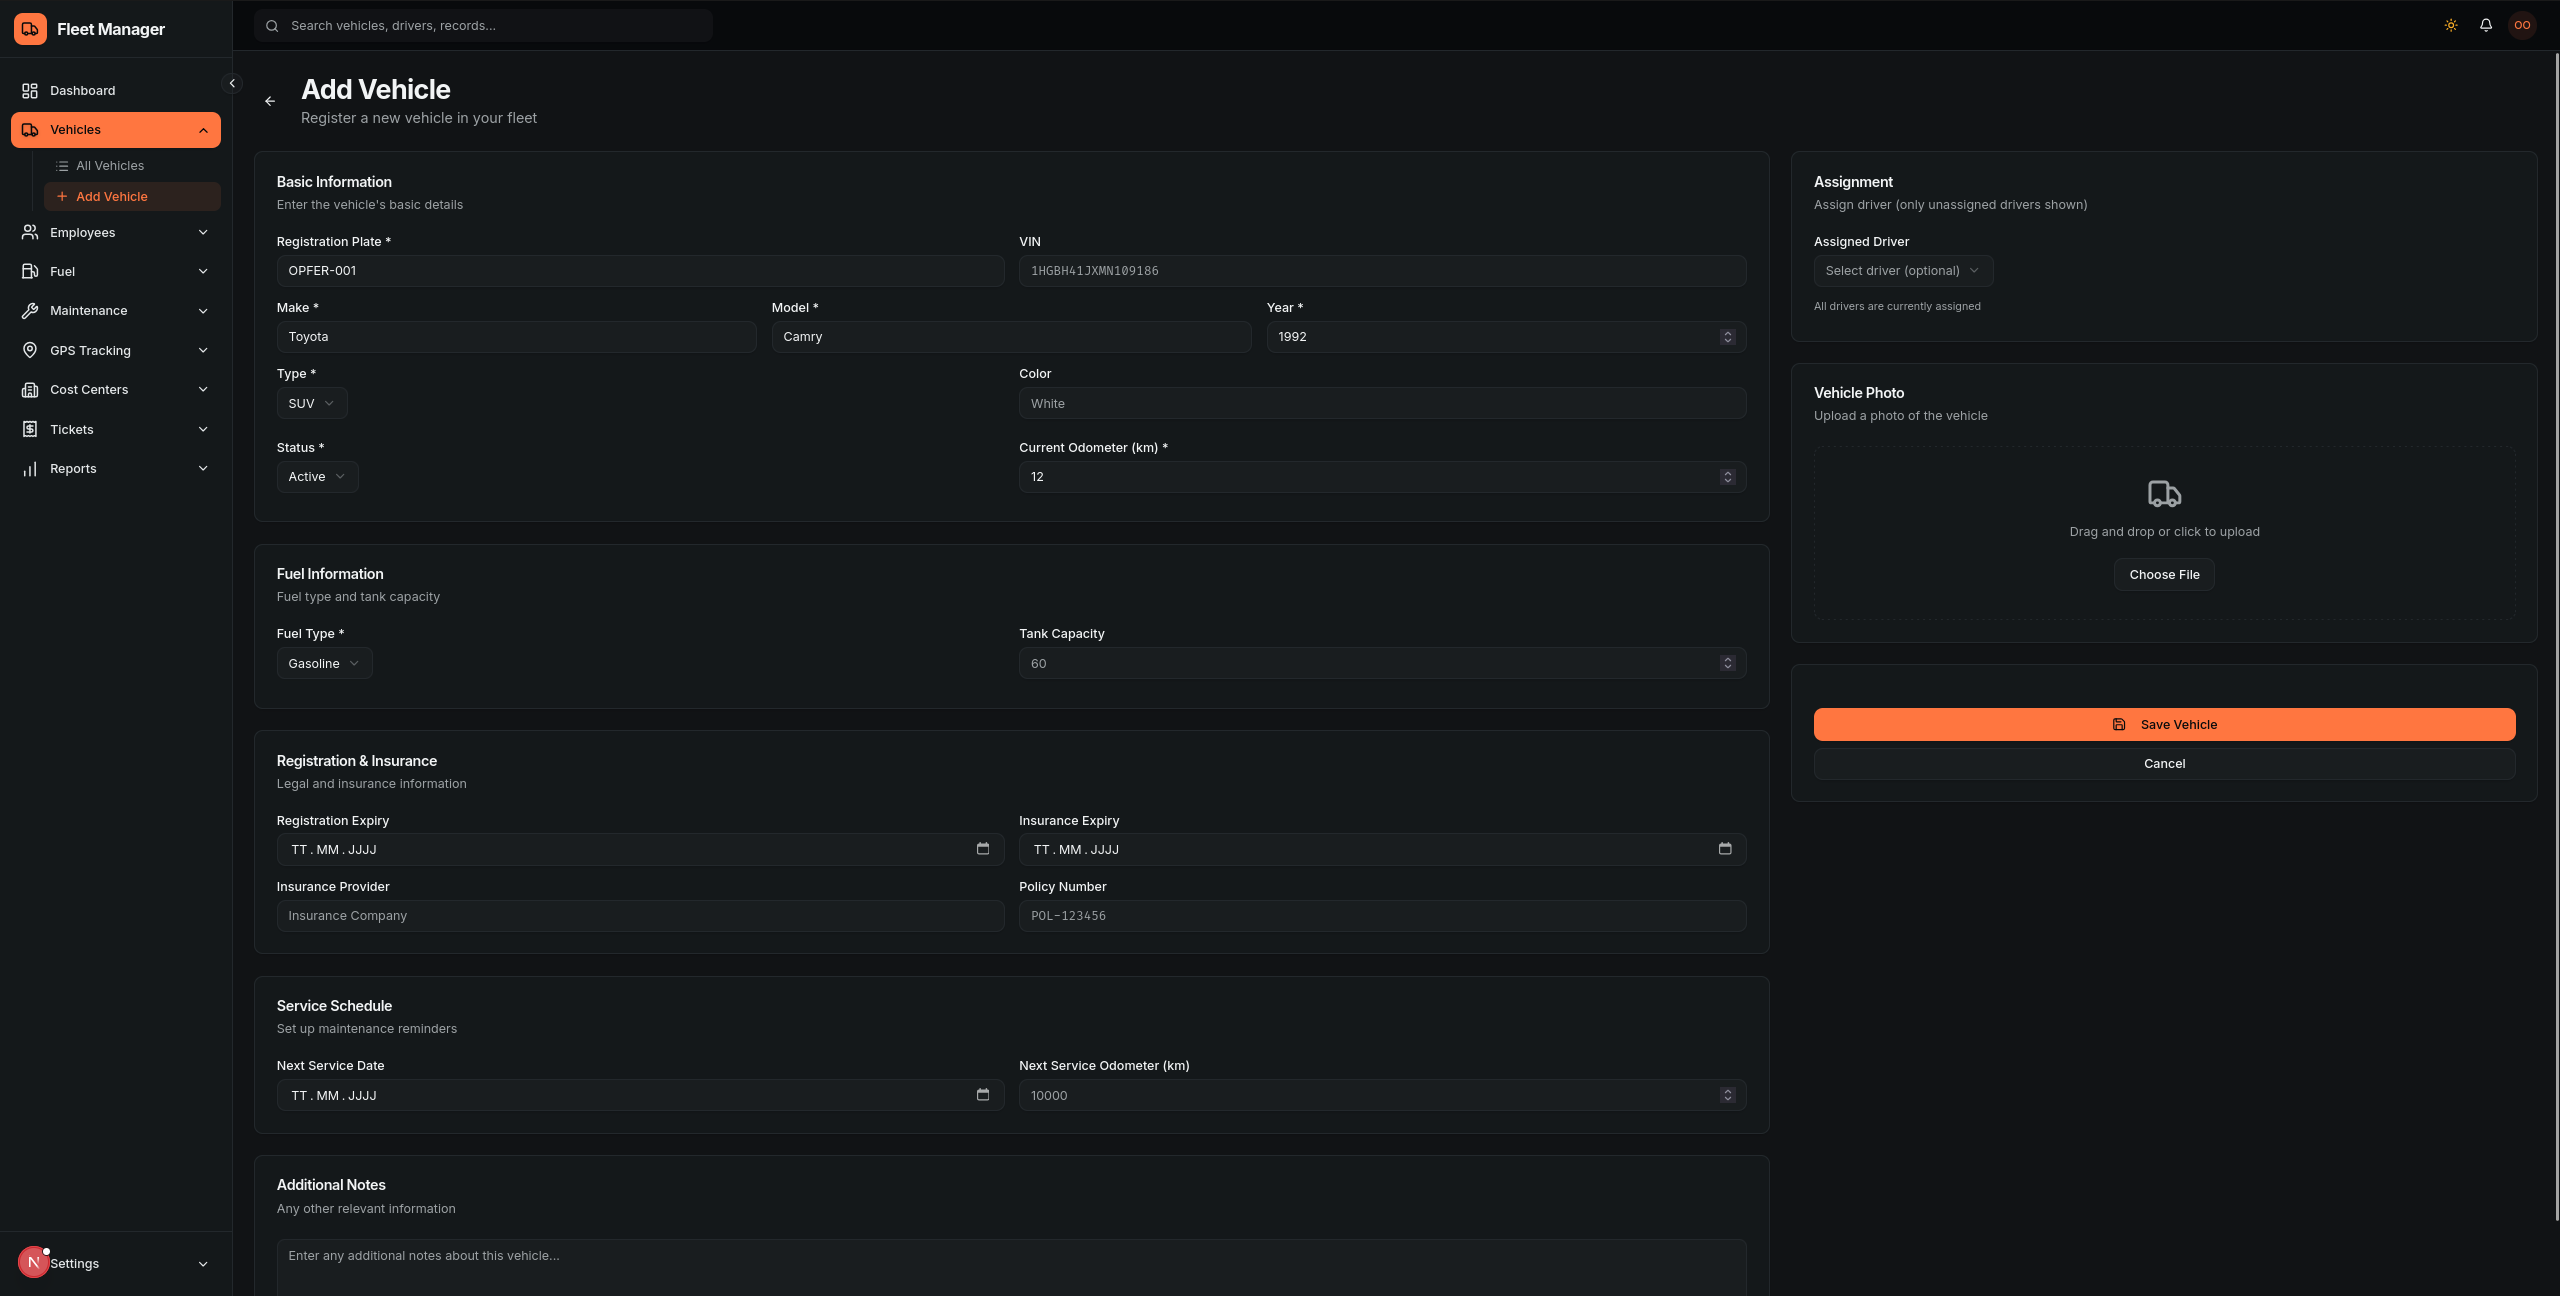
\includegraphics[width=0.9\linewidth]{graphics/ui_attack/opfer_create_vehicle.png}
        \caption{Das Opfer legt im Fleet-Management ein Fahrzeug an.}
        \label{fig:ui-opfer-create-vehicle}
    \end{figure}

    \begin{figure}[H]
        \centering
        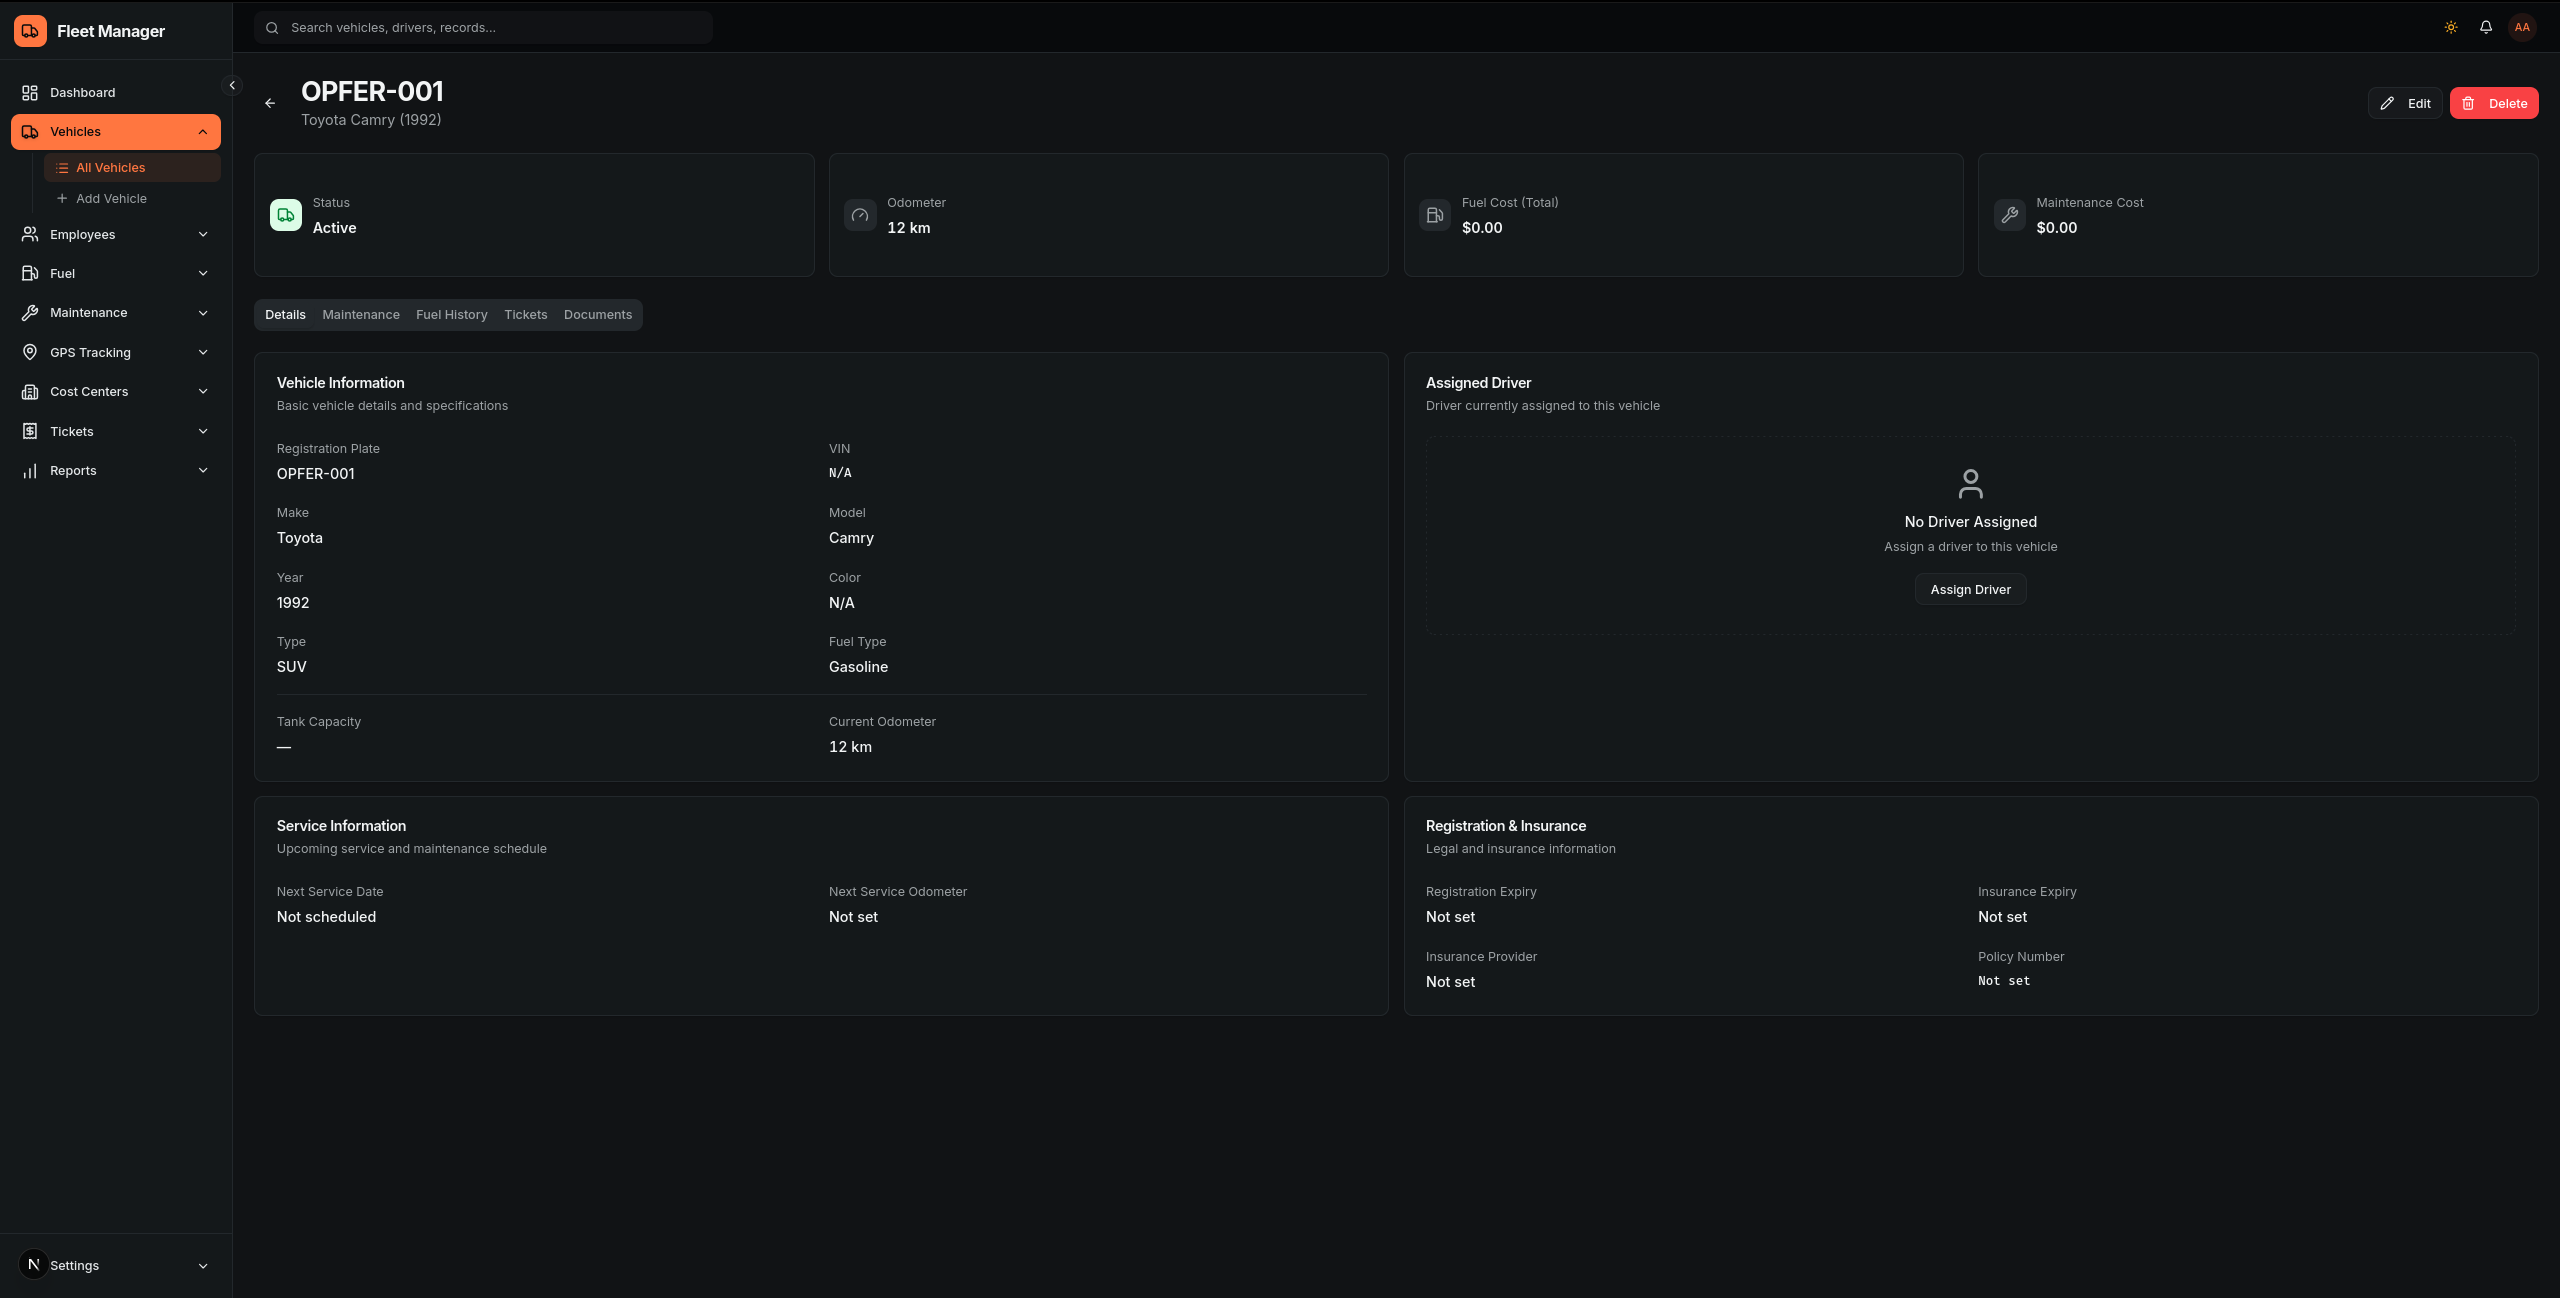
\includegraphics[width=0.9\linewidth]{graphics/ui_attack/angreifer_opfer_vehicle.png}
        \caption{Der Angreifer kann das Fahrzeug des Opfers über die direkte Objekt-ID aufrufen.}
        \label{fig:ui-angreifer-opfer-vehicle}
    \end{figure}

    \begin{figure}[H]
        \centering
        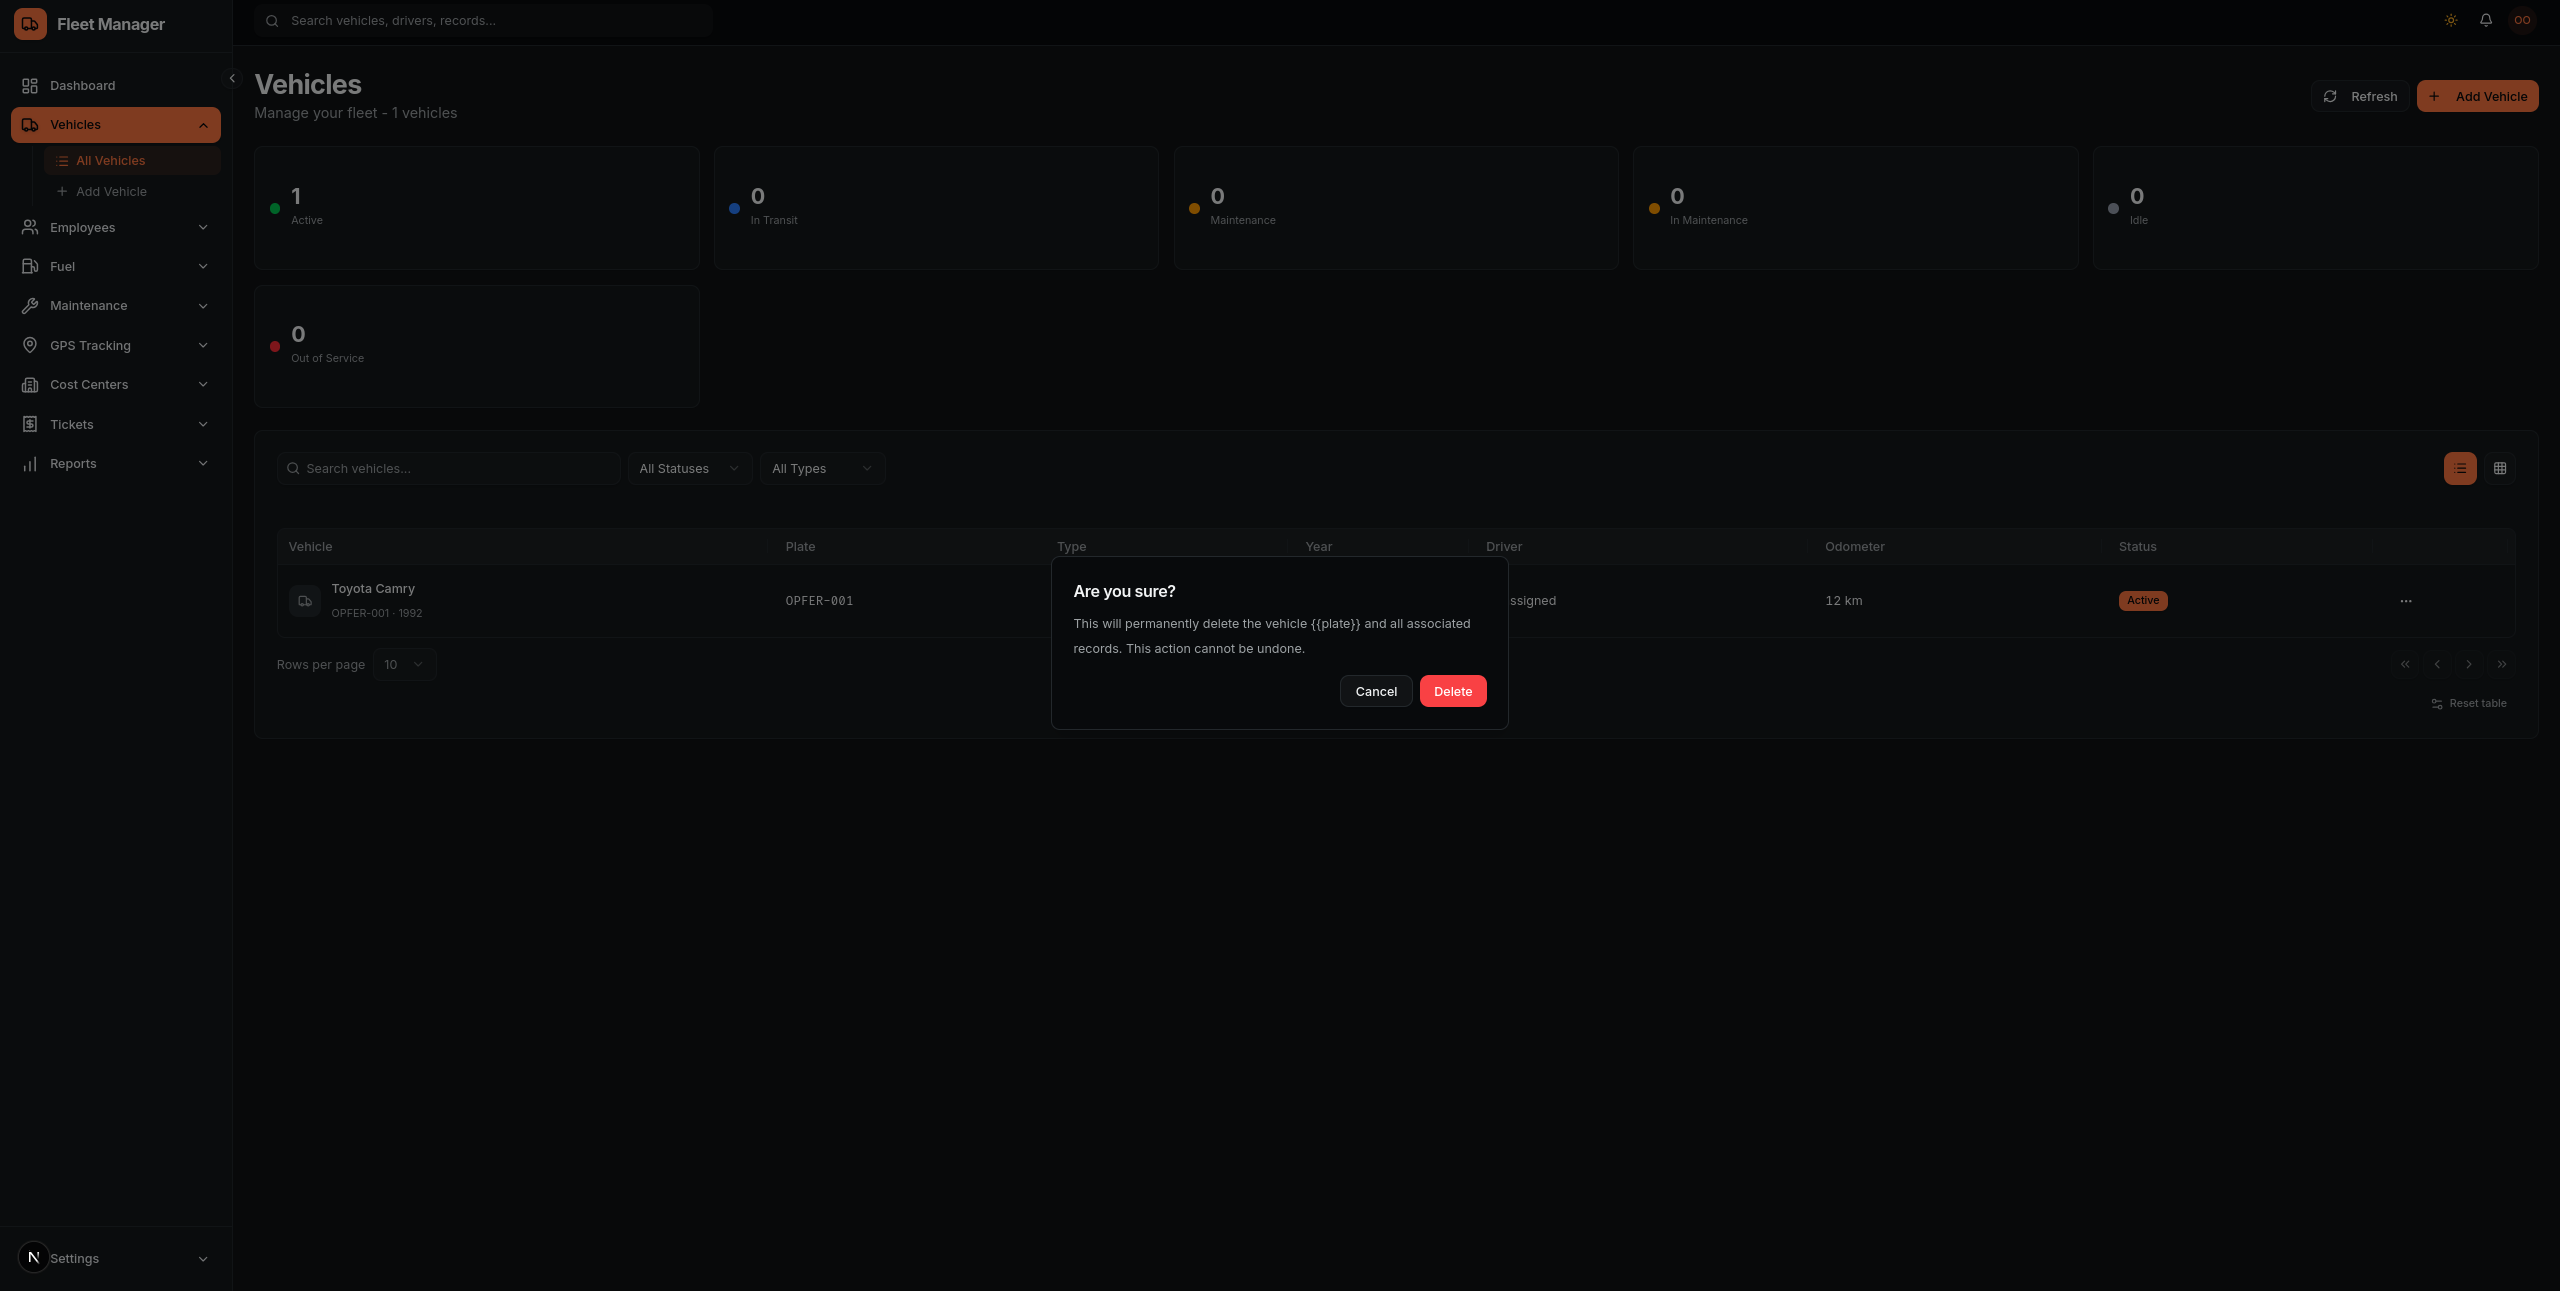
\includegraphics[width=0.9\linewidth]{graphics/ui_attack/opfer_softdelete.png}
        \caption{Soft-gelöschte Datensätze bleiben vor dem Patch in der Oberfläche weiterhin erreichbar.}
        \label{fig:ui-softdelete}
    \end{figure}

    \subsection{API-Reproduktion mit curl}

    Die \texttt{curl}-Screenshots zeigen denselben Sachverhalt ohne Frontend. Dadurch
    ist klar erkennbar, dass es sich nicht um ein Anzeigeproblem des Clients,
    sondern um einen serverseitigen Autorisierungsfehler handelt. Das Opfer erzeugt
    ein Fahrzeug, der Angreifer nutzt dessen UUID für einen fremden GET- und
    DELETE-Zugriff, und das Objekt bleibt sogar nach einem Soft-Delete direkt per ID
    lesbar.

    \begin{figure}[H]
        \centering
        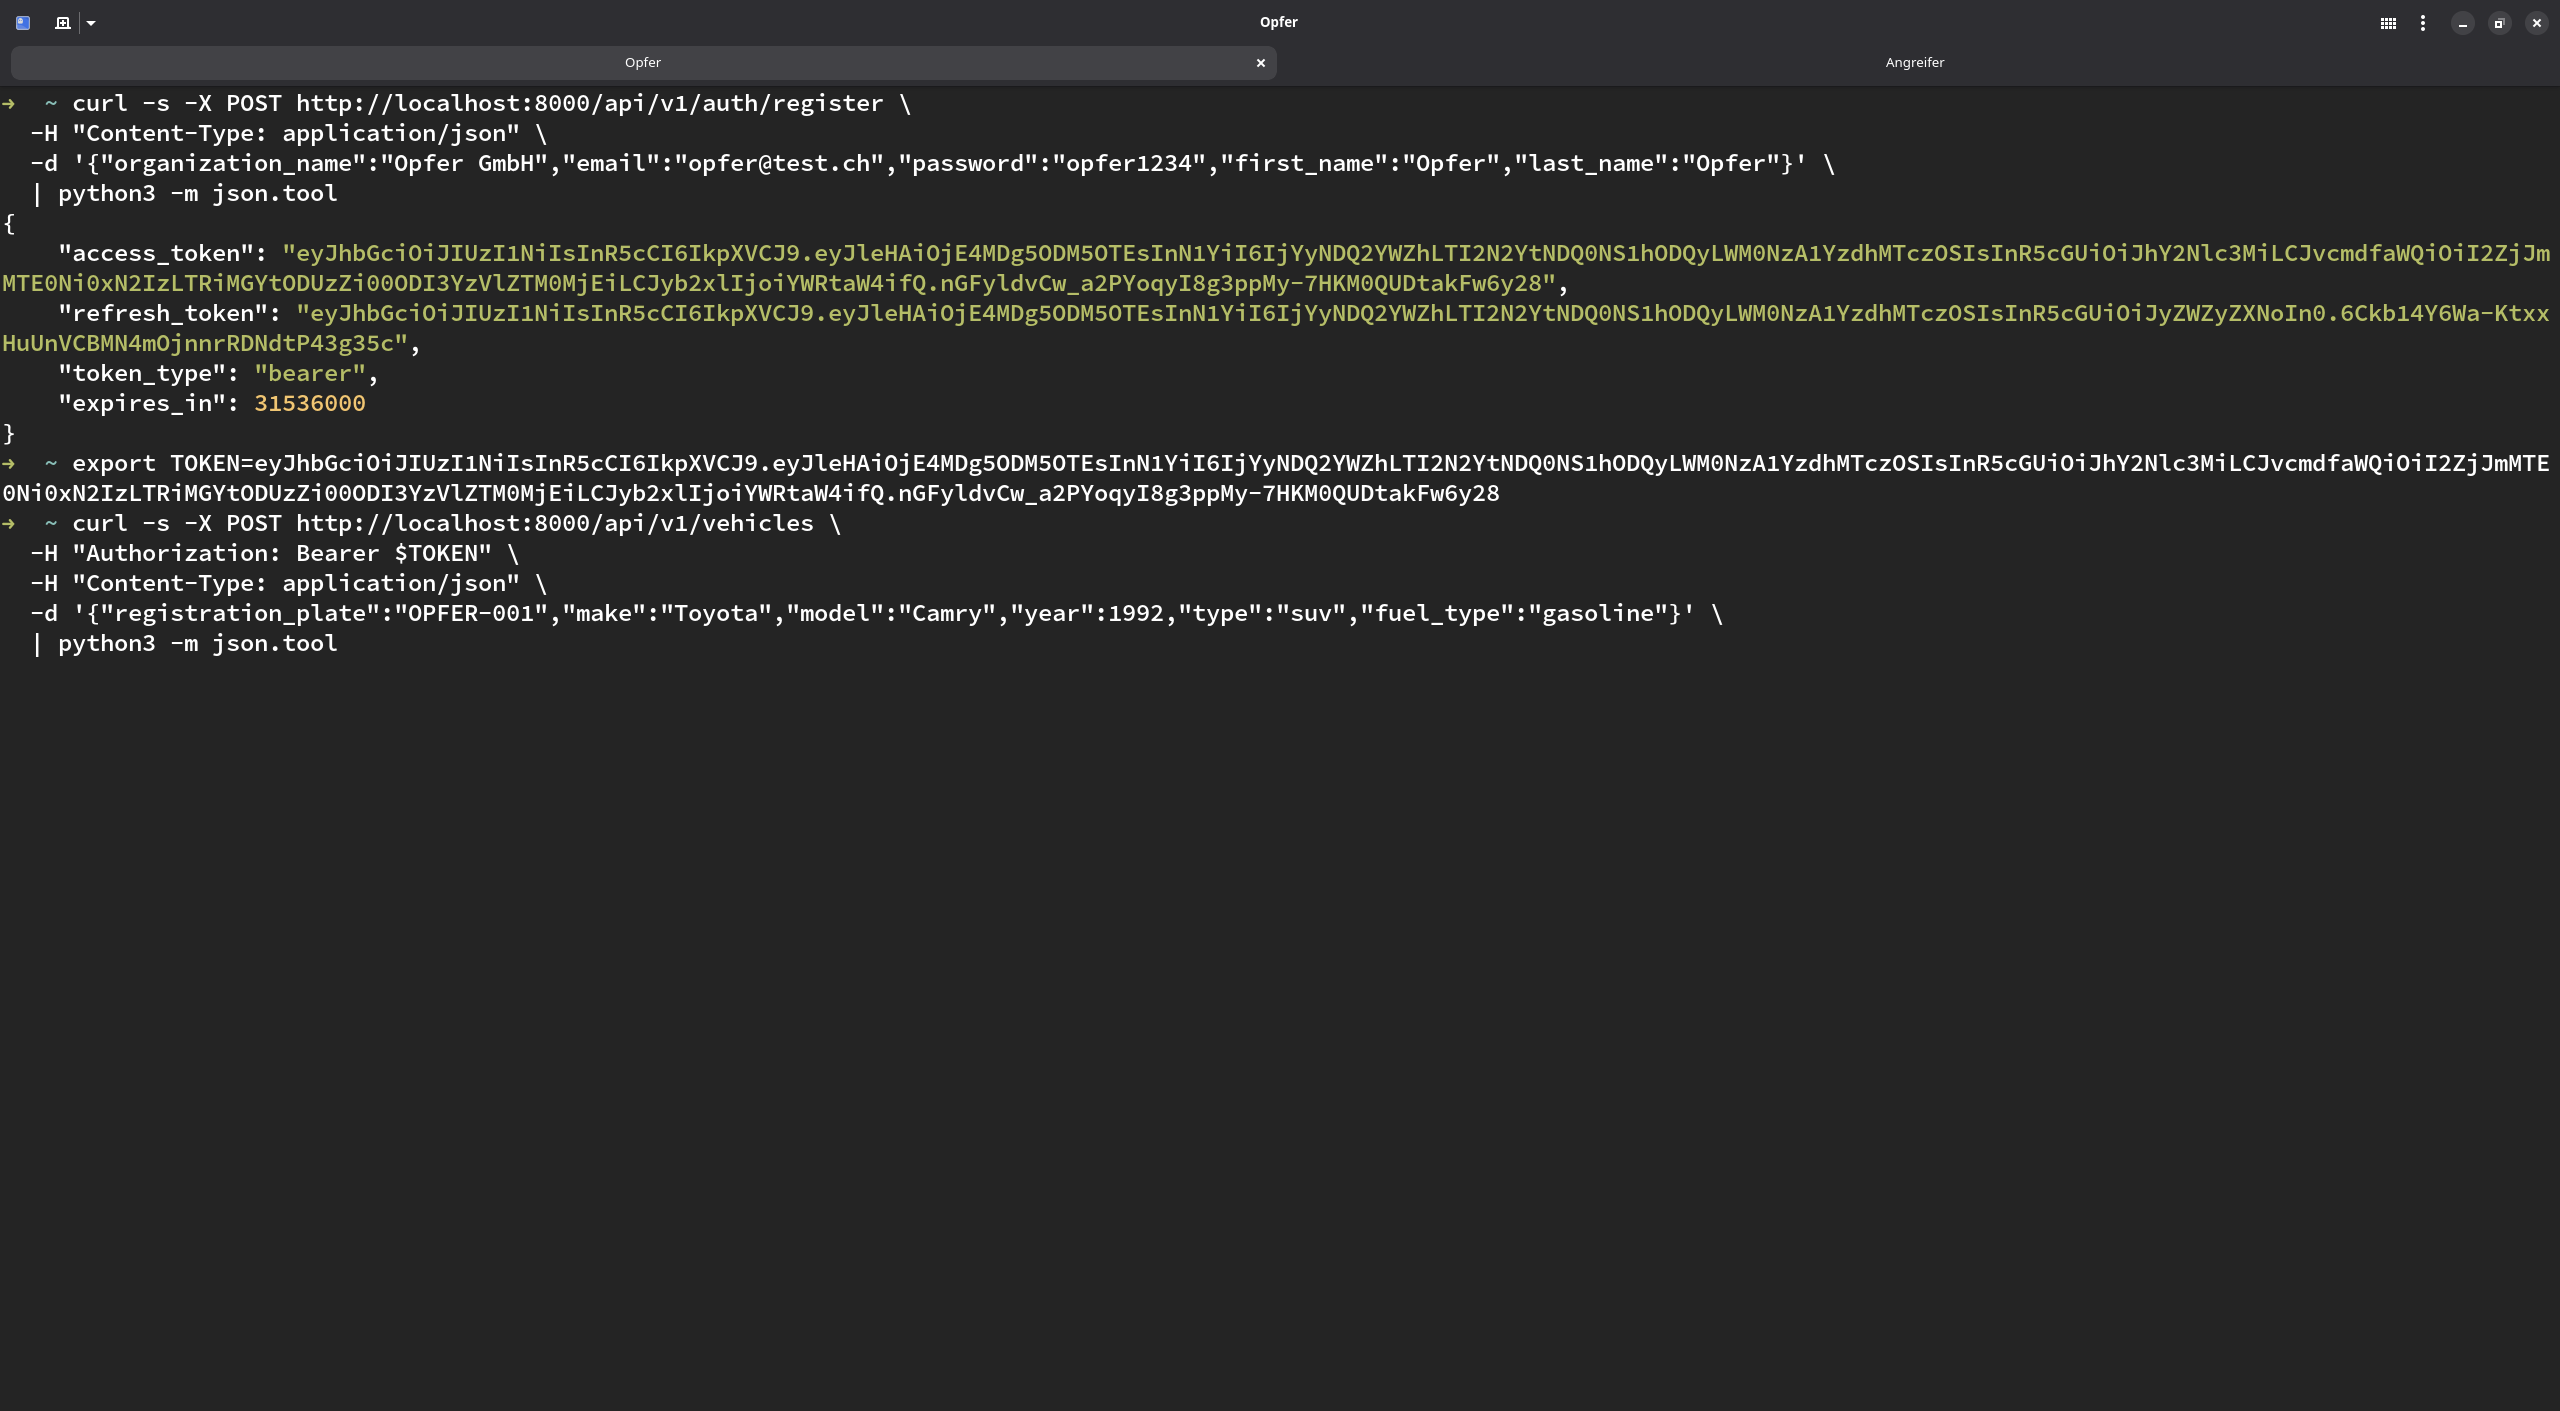
\includegraphics[width=0.9\linewidth]{graphics/curl_attack/opfer_create_vehicle.png}
        \caption{Erzeugung eines Fahrzeugs im Kontext des Opfers per API.}
        \label{fig:curl-opfer-create-vehicle}
    \end{figure}

    \begin{figure}[H]
        \centering
        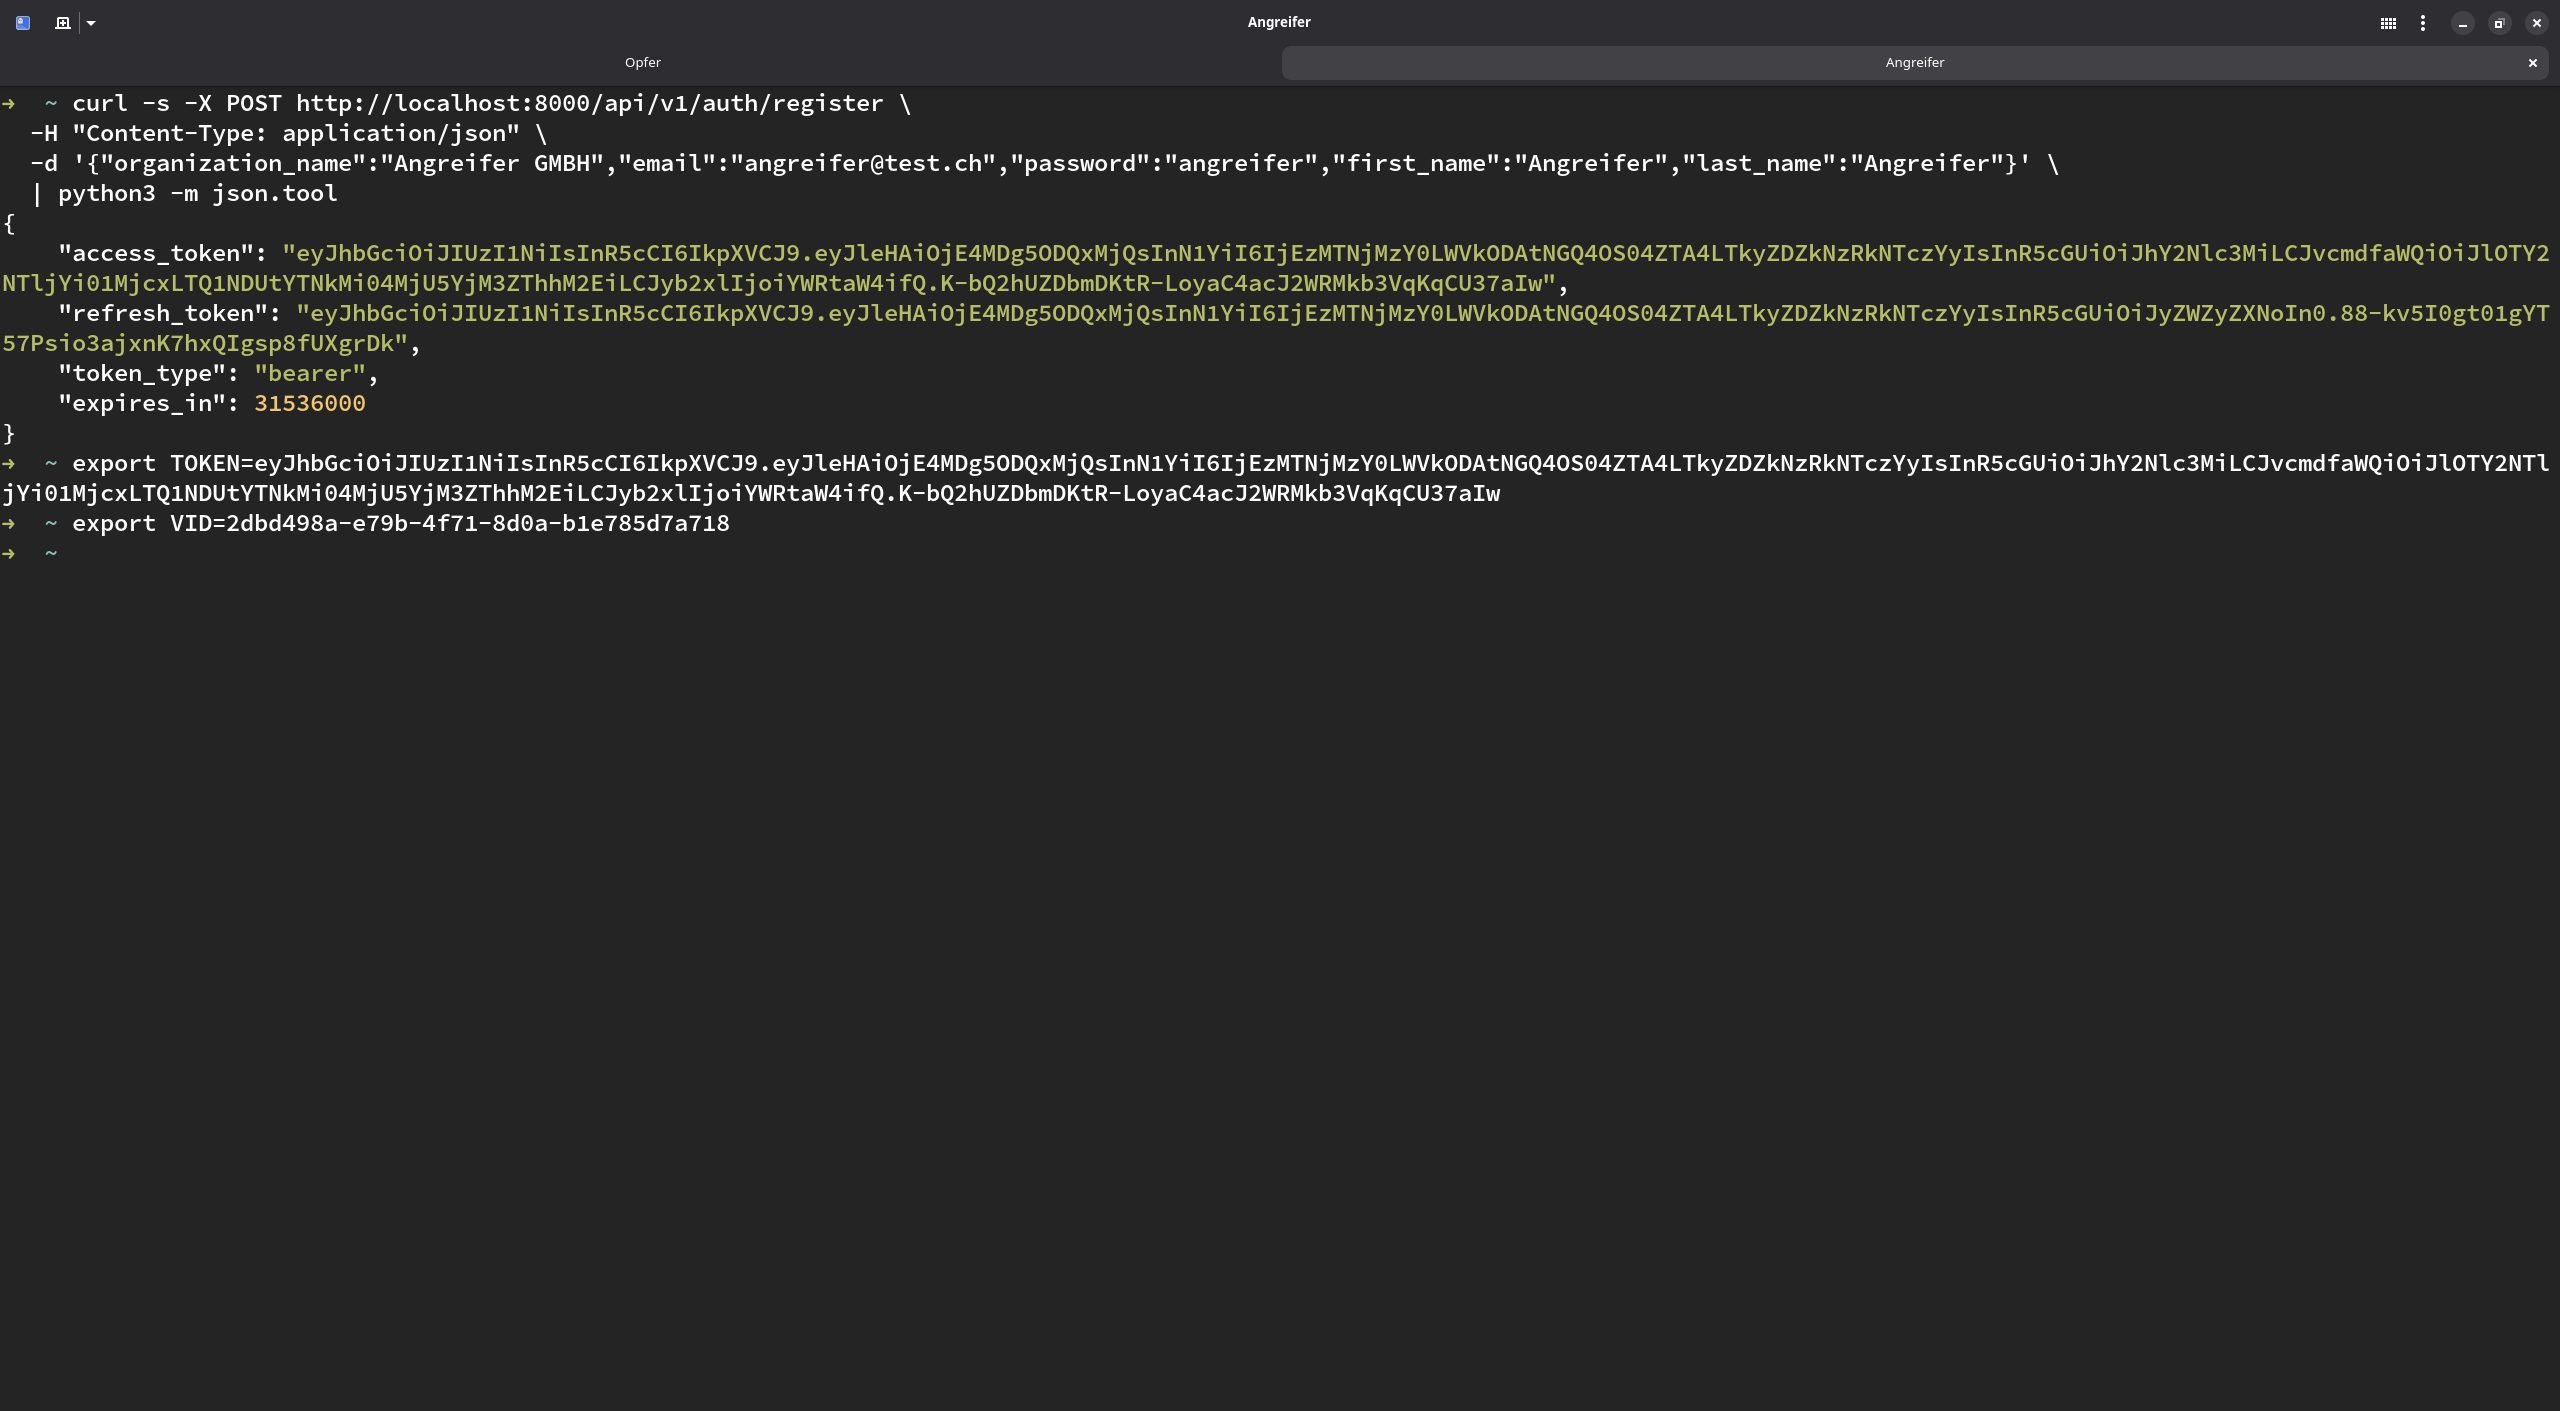
\includegraphics[width=0.9\linewidth]{graphics/curl_attack/use_vehicle_id.png}
        \caption{Der Angreifer verwendet dieselbe UUID für einen unautorisierten GET-Zugriff.}
        \label{fig:curl-use-vehicle-id}
    \end{figure}

    \begin{figure}[H]
        \centering
        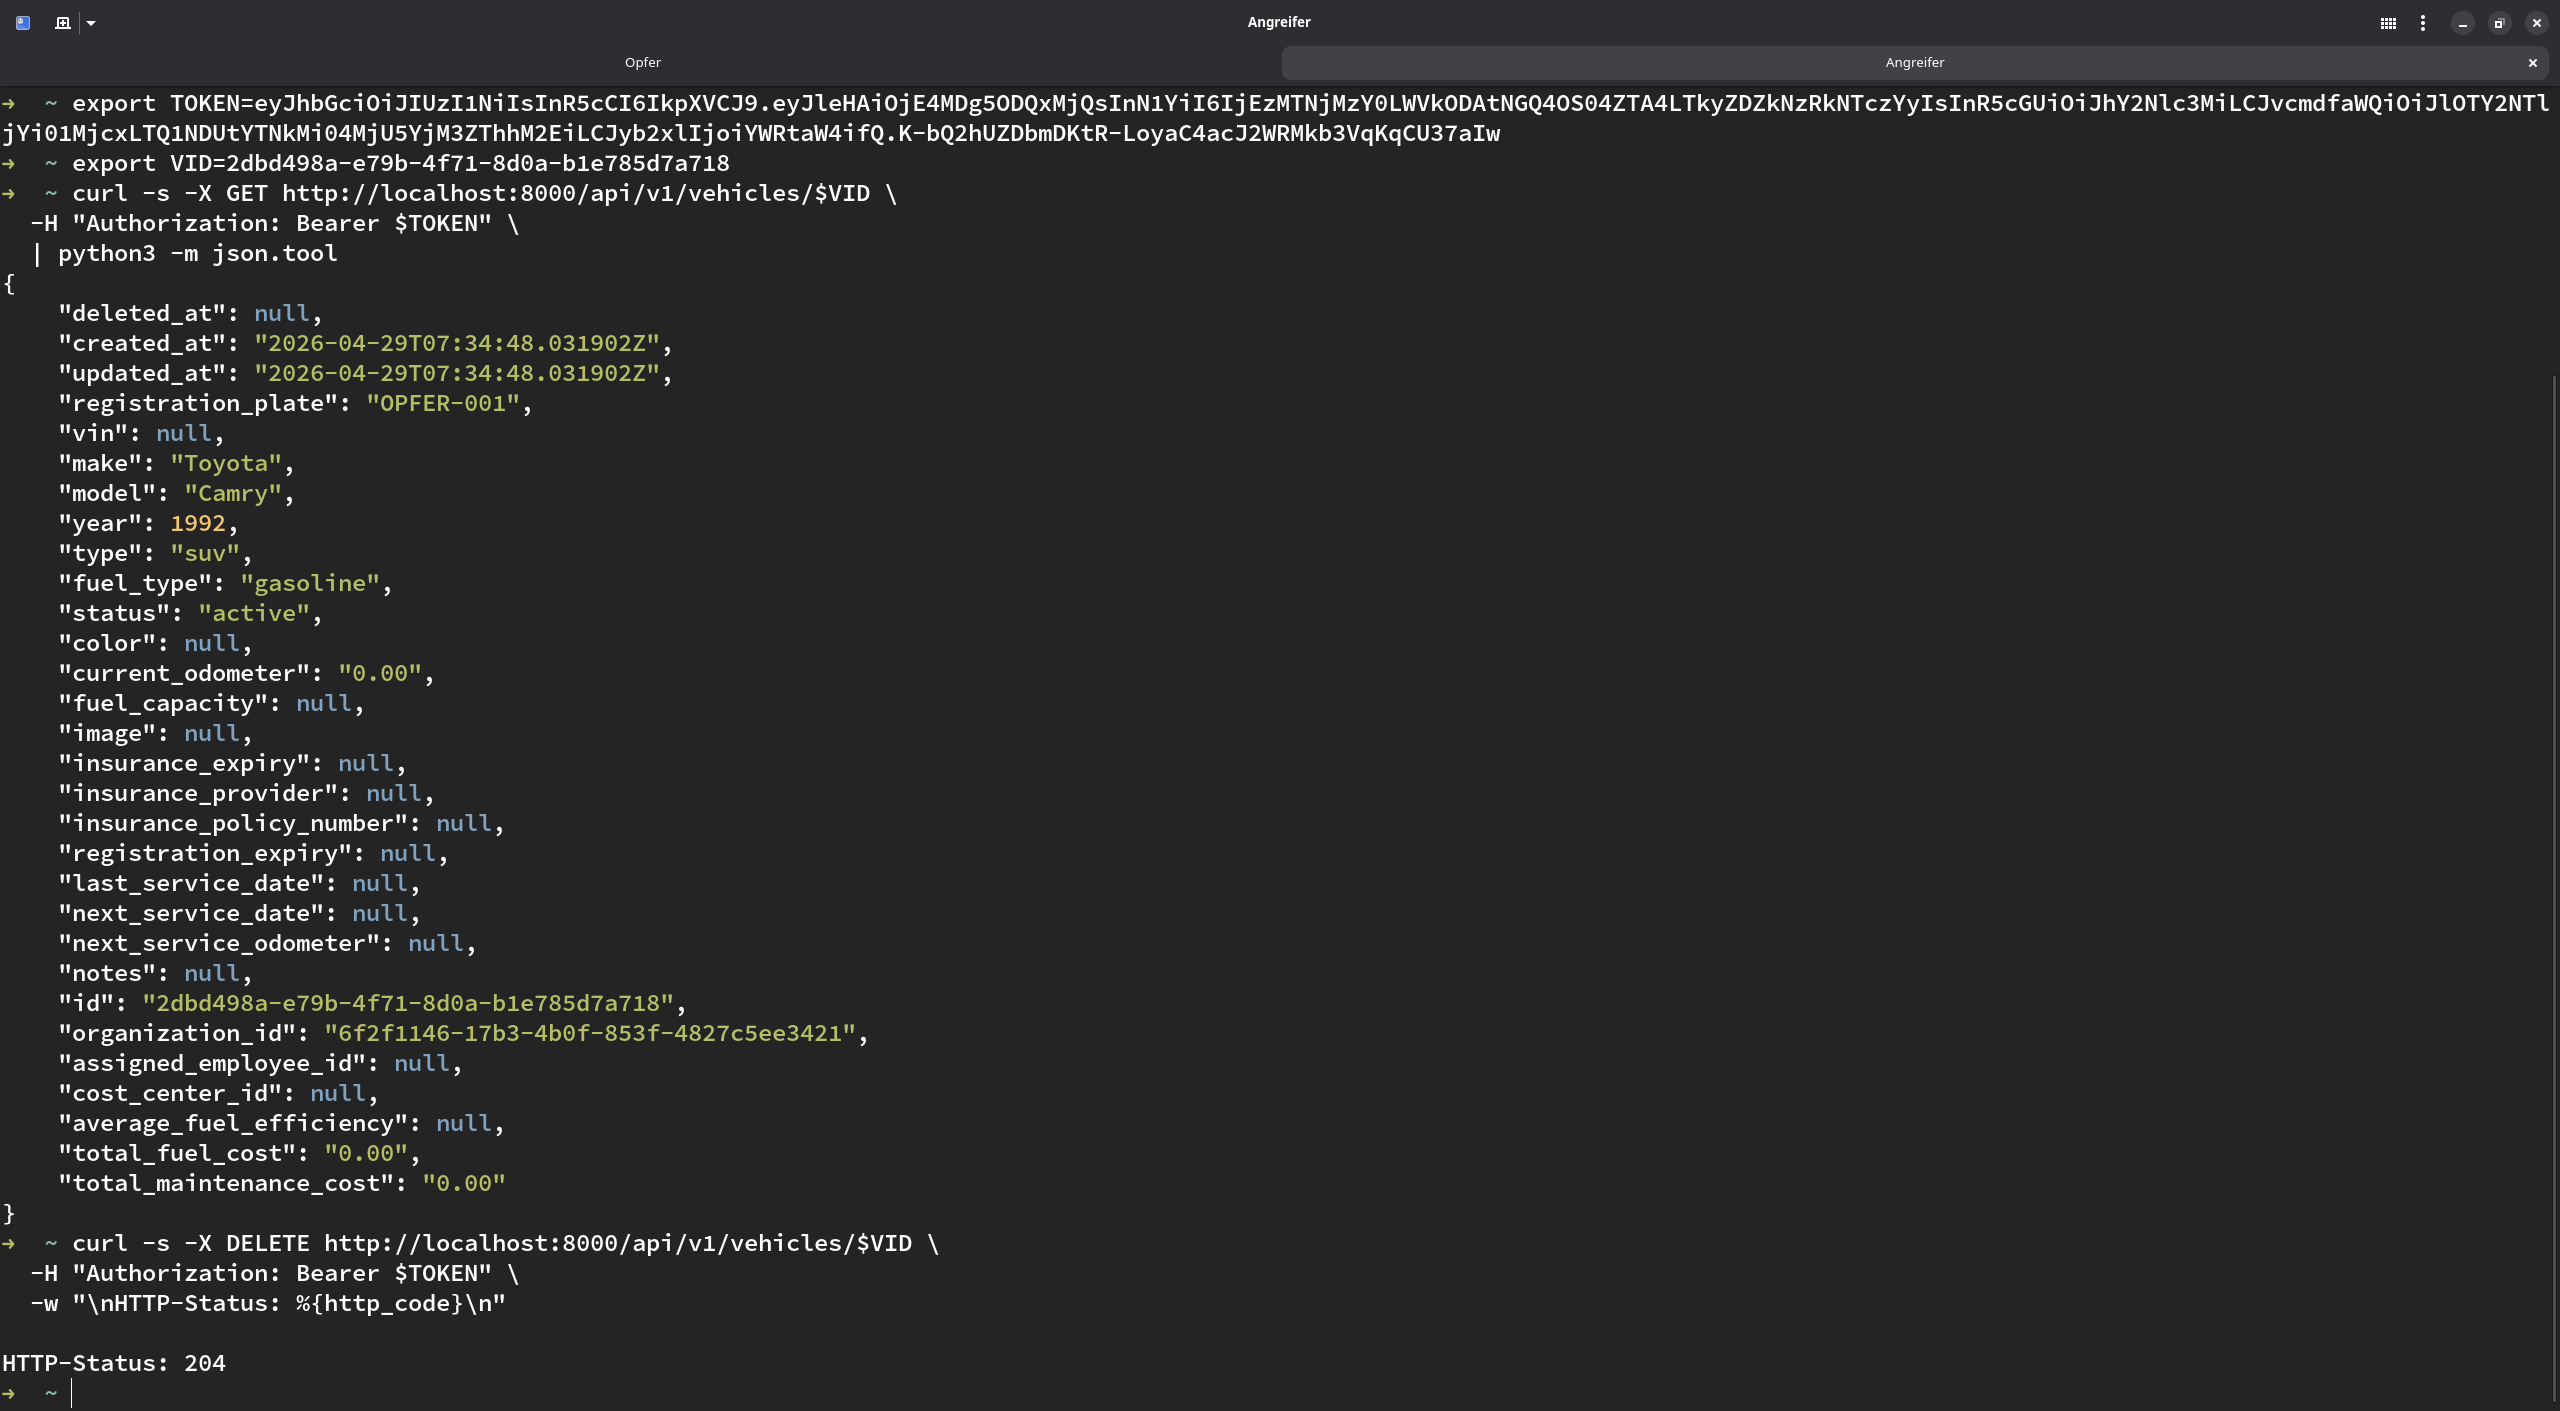
\includegraphics[width=0.9\linewidth]{graphics/curl_attack/angreifer_delete_vehicle.png}
        \caption{Unautorisierter DELETE-Aufruf des Angreifers gegen das Fahrzeug des Opfers.}
        \label{fig:curl-delete-vehicle}
    \end{figure}

    \begin{figure}[H]
        \centering
        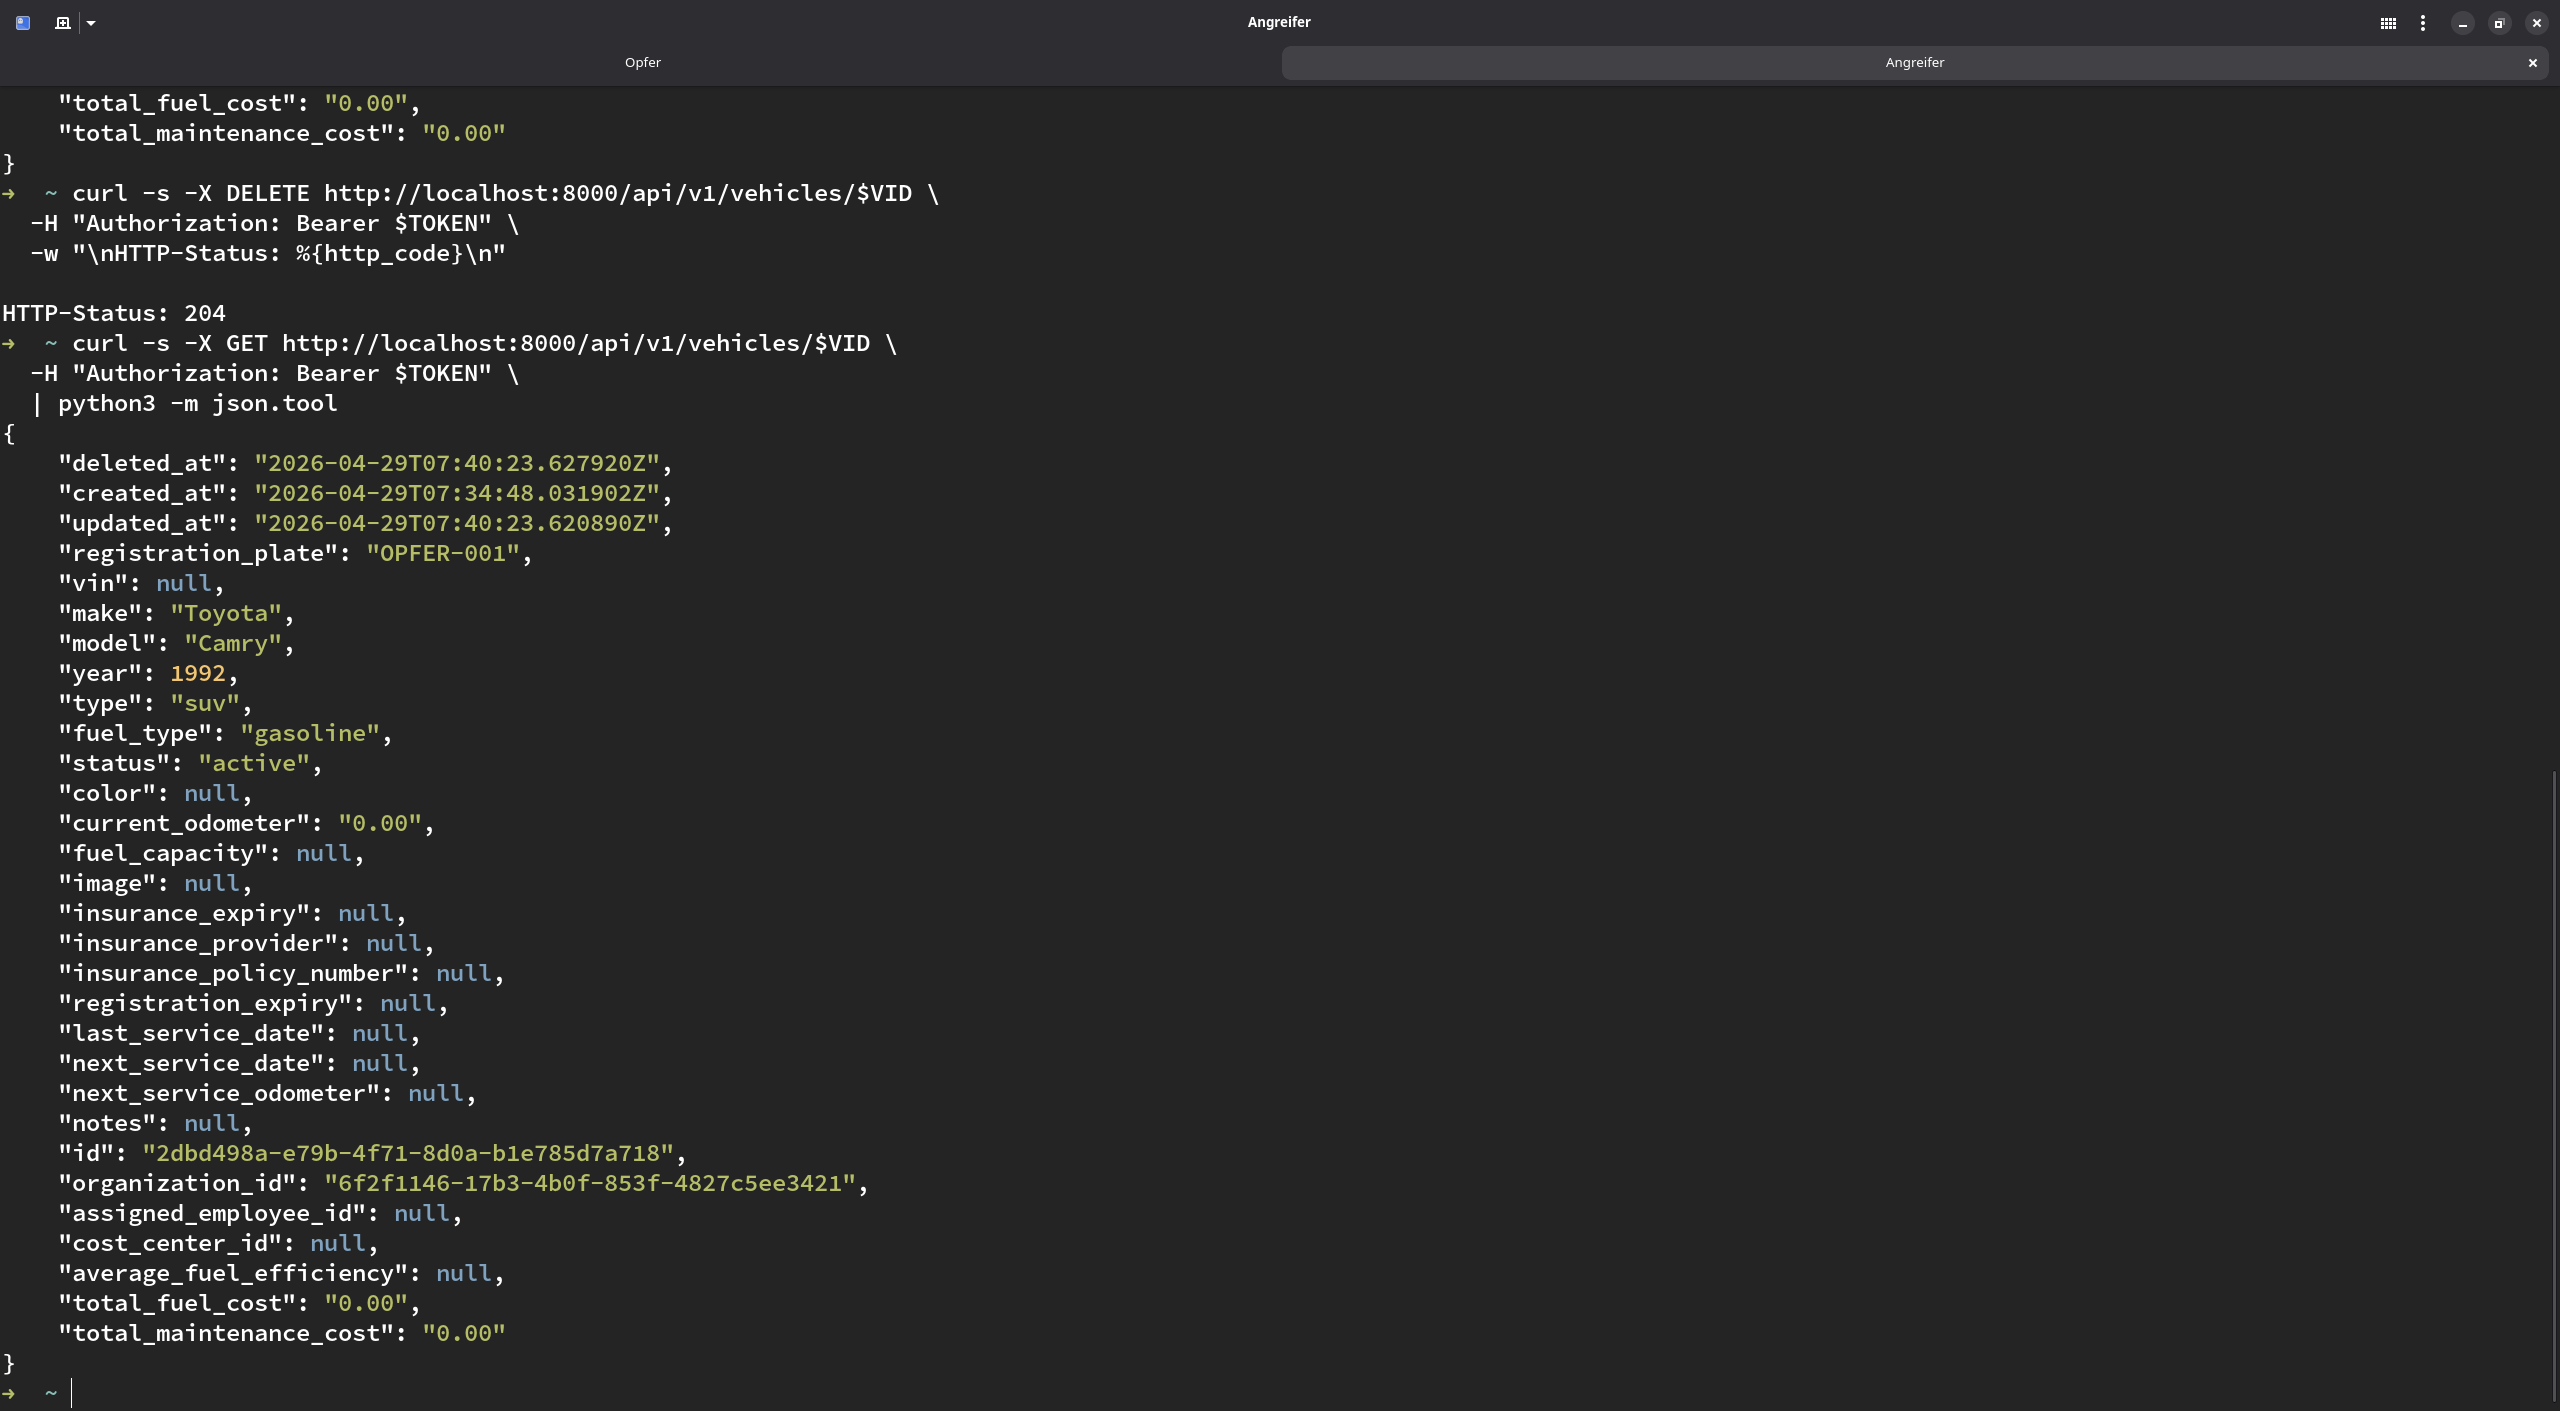
\includegraphics[width=0.9\linewidth]{graphics/curl_attack/vahicle_after_delete.png}
        \caption{Das soft-gelöschte Fahrzeug bleibt vor dem Patch per direkter ID-Abfrage sichtbar.}
        \label{fig:curl-vehicle-after-delete}
    \end{figure}

    %\includepdf[pages={1-2},nup=1x2,landscape=true,scale=0.85,offset=10 -40,pagecommand={\section{Eingefügtes Dokument; zwei Seiten auf einer}\label{app:Aufgabenstellung}\thispagestyle{myheadings}}]{appendix/aufgabenstellung.pdf} \newpage

    %%Bei mehrseitigen Dokumenten die folgenden Seiten ohne Überschrift:
    %\includepdf[pages={3-6},nup=1x2,landscape=true,scale=0.85,offset=10 -40,pagecommand={\thispagestyle{myheadings}}]{appendix/aufgabenstellung.pdf} \newpage

    %\includepdf[pages={1},nup=1x1,landscape=true,scale=0.85,offset=10 -40,pagecommand={\section{Eingefügte PDF-Tabelle}\label{app:Timetable}\thispagestyle{myheadings}}]{appendix/timeline_example.pdf} \newpage

    %%Bei mehrseitigen Dokumenten die folgenden Seiten ohne Überschrift:
    %\includepdf[pages={2-5},nup=1x1,landscape=true,scale=0.85,offset=0 -20,pagecommand={\thispagestyle{myheadings}}]{appendix/timeline_example.pdf} \newpage

\end{appendix}


%%---NOTES for DEBUG---------------------------------------------------------------------
%\newpage
%\listoftodos[\section{Todo-Notes}]
%\clearpage

\end{document}